\chapter[A Lighthouse in the Dust]{Reverberation of Doppler Boosted Emission from Massive Black Hole Binaries I: A Lighthouse in the Dust}
\label{ch:Dust}
\let\thefootnote\relax\footnotetext{We dedicate this work to the memory of Arlin Crotts who passed away on November 19, 2015. As an expert on supernovae light echoes, we sorely missed his collaboration on this work.}





\section{Introduction} 
Massive black holes (MBHs) exist at the centers of
most, if not all, galaxies \citep{kr95, KormendyHo2013}. Galactic mergers can
deliver MBHs, as well as an ample supply of gas \citep{BH1992, Barnes:1996,
Barnes:2002, Mayer:2013:MBHBGasRev}, to the centers of newly coalesced
galaxies where the MBHs form a binary. The interaction of massive black hole
binaries (MBHBs) with gas and surrounding stars can drive the pair to sub-pc
separations where gravitational radiation reaction drives the binary to
coalescence \citep{Begel:Blan:Rees:1980}.  Characterization of the population
of such sub-pc binaries, through present electromagnetic (EM), and future
gravitational wave (GW) channels will provide a powerful tool for
understanding the mutual build-up of galaxies and central black holes
\citep[\textit{e.g.}][]{KormendyHo2013}, the dynamics of gas and stars in
galactic nuclei \citep[\textit{e.g.}][]{MerrittMilos:2005:LRR}, and the low-
frequency gravitational wave background
\citep[\textit{e.g.}][]{KocsisSesana:2011, Shannon:2015,
Arzoumanian:2015:SGWB}.

The electromagnetic signatures of MBHBs can arise from their interaction with
gas. Hydrodynamical simulations of gas discs surrounding close MBHBs show that
accretion rates onto a binary can rival, and even exceed the accretion rates
onto a single black hole of an equivalent mass \citep{ShiKrolik:2012,
DHM:2013:MNRAS, Farris:2014, ShiKrolik:2015, MunozLai:2016}. Binary accretion
rates can also be uniquely identifiable. Depending on the ratio of BH masses,
$q \equiv M_2/M_1$ ($M_1>M_2$), the accretion induced emission can be
periodically modulated \citep{Farris:2015:Cool}. For systems with $q \gsim
0.05$, the accretion rate is modulated by the strong perturbations from the
time-dependent binary potential \citep{D'Orazio:CBDTrans:2016}. Periodicity in
the accretion rate, and the resulting luminosity of emission, occur at the
binary orbital period and also twice this period for $0.05 \lsim q \lsim 0.3$.
while for $0.3 \lsim q < 1.0$, an additional periodicity appears at $\sim3
\rightarrow 8\times$ the binary orbital period \citep{ShiKrolik:2012,
DHM:2013:MNRAS, Farris:2014, ShiKrolik:2015, MunozLai:2016}.

In addition to luminosity variations that track accretion rate variability,
luminosity variations will occur due to special relativity alone. For binary
components moving at relativistic speeds (greater than a few $\%$ the speed of
light), any emission will vary in brightness at the period of the binary orbit
due to Doppler boosting \citep{PG1302MNRAS:2015a,
PG1302Nature:2015b}.\footnote{For equal mass binaries on circular orbits, each
BH emits at the same luminosity and moves at the same orbital speed, hence
Doppler boosting effects are nullified unless one BH can accrete at a higher
rate than the other; such a scenario may occur for eccentric binaries
\citep{MunozLai:2016}.}  For binaries with disparate mass ratios, $q \lsim
0.05$, accretion is steady and dominated by the smaller, secondary BH
\citep{DHM:2013:MNRAS, Farris:2014}. In this case, Doppler boosting is expected
to be the primary, if not only, source of variability. Even near-equal mass
binaries, for which high levels of accretion variability are expected, may
emit steadily in their rest frame: If viscous and tidal forcing timescales
which transport matter from the edges of the mini-disks around each BH down to
the BH inner most stable circular orbit are long compared to accretion rate
changes at the mini-disc edges, then luminosity variations may be muted by
buffering in the mini-disks. In this case too, Doppler boosting will be the
dominate source of variability from accreting MBHBs.



The Doppler boosting scenario has recently been developed to interpret the
MBHB candidate PG 1302-102 \citep{Graham+2015a}, which exhibits a nearly
sinusoidal periodicity in the V-band continuum. Given the measured binary
mass, period, and spectral slope of PG 1302, \cite{PG1302Nature:2015b} showed
that the observed amplitude of variability in the V-band and ultra-violet (UV)
wavelengths is consistent with that expected for Doppler boosting of emission
from an accretion disk around the secondary BH. Further confirmation of the
Doppler boosting model for PG 1302 will require continued, long-term
observations of the system in optical and UV wavelengths. However measurements
in other wavelengths can provide additional clues to the nature of the central
engine of PG 1302.

Such clues have recently come from the infrared (IR). \cite{Jun:2015} analyze
data from the WISE satellite to report a periodicity in the IR continuum of PG
1302 which is consistent with the optical period, but with a diminished
amplitude and at a phase lag of $335 \pm 153$ days in the W1 band and $524 \pm
148$ days in the W2 band. \cite{Jun:2015} attribute this phase lag to reprocessing of the
UV/optical continuum of PG 1302 by a surrounding dusty torus at $\sim$pc
distances from the illuminating source.

In this work we develop a toy model to interpret the findings of \cite{Jun:2015} and, in
general, reverberated IR emission from MBHBs. We considers heating of nuclear
dust by isotropically varying emission from the central source, and compare to
models with spatially, and temporally, varying Doppler boosted binary
emission, illuminating the dust structure as it sweeps around like a
lighthouse at the binary orbital frequency. We crucially take into account the
relative light travel time to different parts of the dust structure in a
smooth dusty-torus model. We find that the relative magnitude and phase lag of
the reverberated IR emission is dependent not only on the size of the dust
region, but also on its geometry and the pattern speed of the variable
illuminating source (the binary orbital period relative to the light travel
time to the dust region). We find also that, for Doppler boosted emission
models, depending on the relative inclination angles of the binary and the
dust torus to the observer's line of sight, variability can be present in both
optical and IR, or in one band and not the other. This means that present
optical surveys of MBHB candidates may have missed some candidates which vary
only in the reverberated IR and motivates and IR plus optical search for
periodic Quasars.


Future work will expand upon the toy models presented here and apply them to
interpret IR emission from the new population of $\gsim100$ MBHB
candidates \citep{Graham+2015b, Charisi+2016} and probe their dusty
environments.



This work is organized as follows. In \S \ref{S:Model} we introduce the MBHB
and dust system. In \S \ref{S:Derivation} we develop models for IR emission
from a dust region heated by both isotropic and Doppler boosted MBHB
continua. In \S \ref{S:PDs} we explore the parameter dependencies in the
model and their consequences, differentiating between isotropic and Doppler
boost scenarios.  In \S \ref{S:Discussion} we summarize our findings and
consider limitations and possible extensions to the model. In \S
\ref{S:conclusions} we conclude.




\section{Model Setup}
 \label{S:Model}
 \subsection{The Dust}

The unification of type I (unobscured) and type II (obscured) active galactic
nuclei (AGN) posits that the difference in AGN types is only the viewing angle
relative to a torus of obscuring dust \citep{Antonucci:1993,
KrolikBegelman:1988}. The properties of AGN dust have been investigated from
high resolution IR imaging as well as modeling of IR spectral energy
distributions (SEDs). High resolution IR imaging puts an upper limit of a few
parsecs on the size of the emitting dust region \citep[see][and references within]{Elitzur:2006}. 
Spectral energy distribution (SED) modeling has put
forth a wide variety of models of optically thin and optically thick, smooth
and clumpy dust distributions of various geometries in order to determine dust
spatial distributions and dust grain size distributions  \citep[see the review by][as well as  \cite{Barvainis:1987,PierKrolikI:1992b, PierKrolikII:1993, LaorDraine:1993, GranatoDanese:1994,  Granato:1997,RowanRobinson:1995,Manske:1998,Nenkova:2002,vanBemmelDullemond:2003, Schartmann:2005, NenkovaI:2008,NenkovaII:2008, HonigII:2010, MorTrakhtenbrot:2011,MorNetzer:2012}]{Netzer:2015:rev}. Neither imaging or SED fitting, however, uniquely determine the dust properties.



We do not hope to reproduce the full SEDs of AGN dust tori. Instead we aim to
demonstrate the effects of an anisotropic and periodically variable continuum
source on the reverberated IR continuum. Hence, for simplicity, we assume an
infinitely thin shell of dust which absorbs all UV/optical radiation incident
upon it, but is optically thin to its own emission.


% smooth dust distribution of uniform size grains requiring only that the
% density be monotonically decreasing away from the central source and
% distributed in a torus geometry (see below). We work in both the optically
% thin and optically thick limits.



%The dust grain size distribution can be included as a free parameter, and the
%global density distribution can be easily modified within our model. The
%inclusion of dust emission and absorption features \citep[\textit{e.g.} $9.7
%\mu$m and $18 \mu$m emission silicate features][]{} could be included with
%further radiative transfer modeling. We proceed by considering the
%reprocessing of light from a central source of optical and UV continuum by a
%smooth dusty torus with the above, simplified properties.




\subsection{MBHB Central Source} 

The central source of UV and optical continuum which heats the dust and causes
it to emit in IR is accretion induced emission from a close MBHB. For BH
masses ranging from $10^5 \rightarrow 10^{10} \Msun$, the specific luminosity
emitted from a steady- state accretion disc has a modified blackbody spectrum
that peaks in the X-ray (lower mass BHs) to the optical (higher mass BHs)
\citep{SS73, TanakaMenou:2010}, which can be efficiently absorbed to heat
$\mu$m size dust particles (see below). Here we are interested in the effect
of variable emission from the MBHB.

First consider a MBHB system for which steady emission is generated in the
rest frame of the smaller BH.\footnote{For example, a MBHB with a disparate binary mass
ratio $q \lsim0.05$ can exhibit steady accretion dominated by the smaller BH
\citep{Farris:2014}.} For binaries with large orbital velocities (a few
percent the speed of light), the steady emission will appear to vary for an
observer that sees a changing line of sight velocity $v_{||}$ of the emitting
secondary. This variation of the observed flux $F^{\rm{obs}}_{\nu}$ is given
by the relativistic Doppler formula,
\begin{equation}
F^{\rm{Dop}}_{\nu} = \frac{F^0_{\nu}}{\left[\gamma\left( 1 - \frac{v_{||}}{c}\right)\right]^{\alpha_{\nu} - 3}},
\label{Eq:Dop1}
\end{equation}
where $c$ is the speed of light, $\gamma = \left[ 1 - (v/c)^2 \right]^{-1/2}$
is the Lorenz factor of the moving source, $v_{||}$ is the projection of the
source velocity into the observer's line of sight $\alpha_{\nu}$ is the
spectral slope of the observed spectrum at frequency $\nu$, $\alpha_{\nu} =
d\rm{ln}F_{\nu} / d \rm{ln}\nu$, and we assume that in a given observational
frequency band the rest frame specific flux is a power law in frequency
$F^0_{\nu} \propto \nu^{\alpha_{\nu}}$. Assuming a flat spectrum in frequency
space $\alpha=0.0$, an edge-on view of the binary, and a mass ratio of
$q=0.05$, Figure \ref{Fig:boostParams} shows the combinations of MBHB periods,
and masses for which the secondary orbital velocity can cause a significant
modulation in the observed light curve. MBHBs with orbital periods of a
few years and total masses of $\geq 10^8 \Msun$ will cause $\geq 0.1$ mag
modulations due to Doppler boosting.

In what follows we consider the heating of dust grains by the Doppler
modulated emission. This gives rise to a variable feature in the reprocessed
IR which does not necessarily track the optical and UV continuum, but shares
the same period.

To isolate the effects of the Doppler boosted source emission on the IR
emission, we also consider a control source, which varies isotropically as a
sinusoid in time,
\begin{equation}
F^{\rm{Iso}}_{\nu} = F^0_{\nu}\left[ 1 + A \sin{\Omega \left( t - t_0\right)} \right],
\label{Eq:Iso1}
\end{equation}
where $F^0_{\nu}$ is an average flux, A is the amplitude of modulations,
$P=2\pi / \Omega$ is the period of modulation, and $t_0$ is the relative
phase. This variable source flux is also representative of other sources of
variability, due to variable accretion rates, or intrinsic Quasar variability.

 %%%%%%%%%%%%%%%%%%%%%%%%%%%%%%%%%%%%%%%%%%%%%%%%
%%% FIGURE: boosting params M and P %%%
%%%%%%%%%%%%%%%%%%%%%%%%%%%%%%%%%%%%%%%%%%%%%%%%
\begin{figure}
\begin{center}$
\begin{array}{c}
%
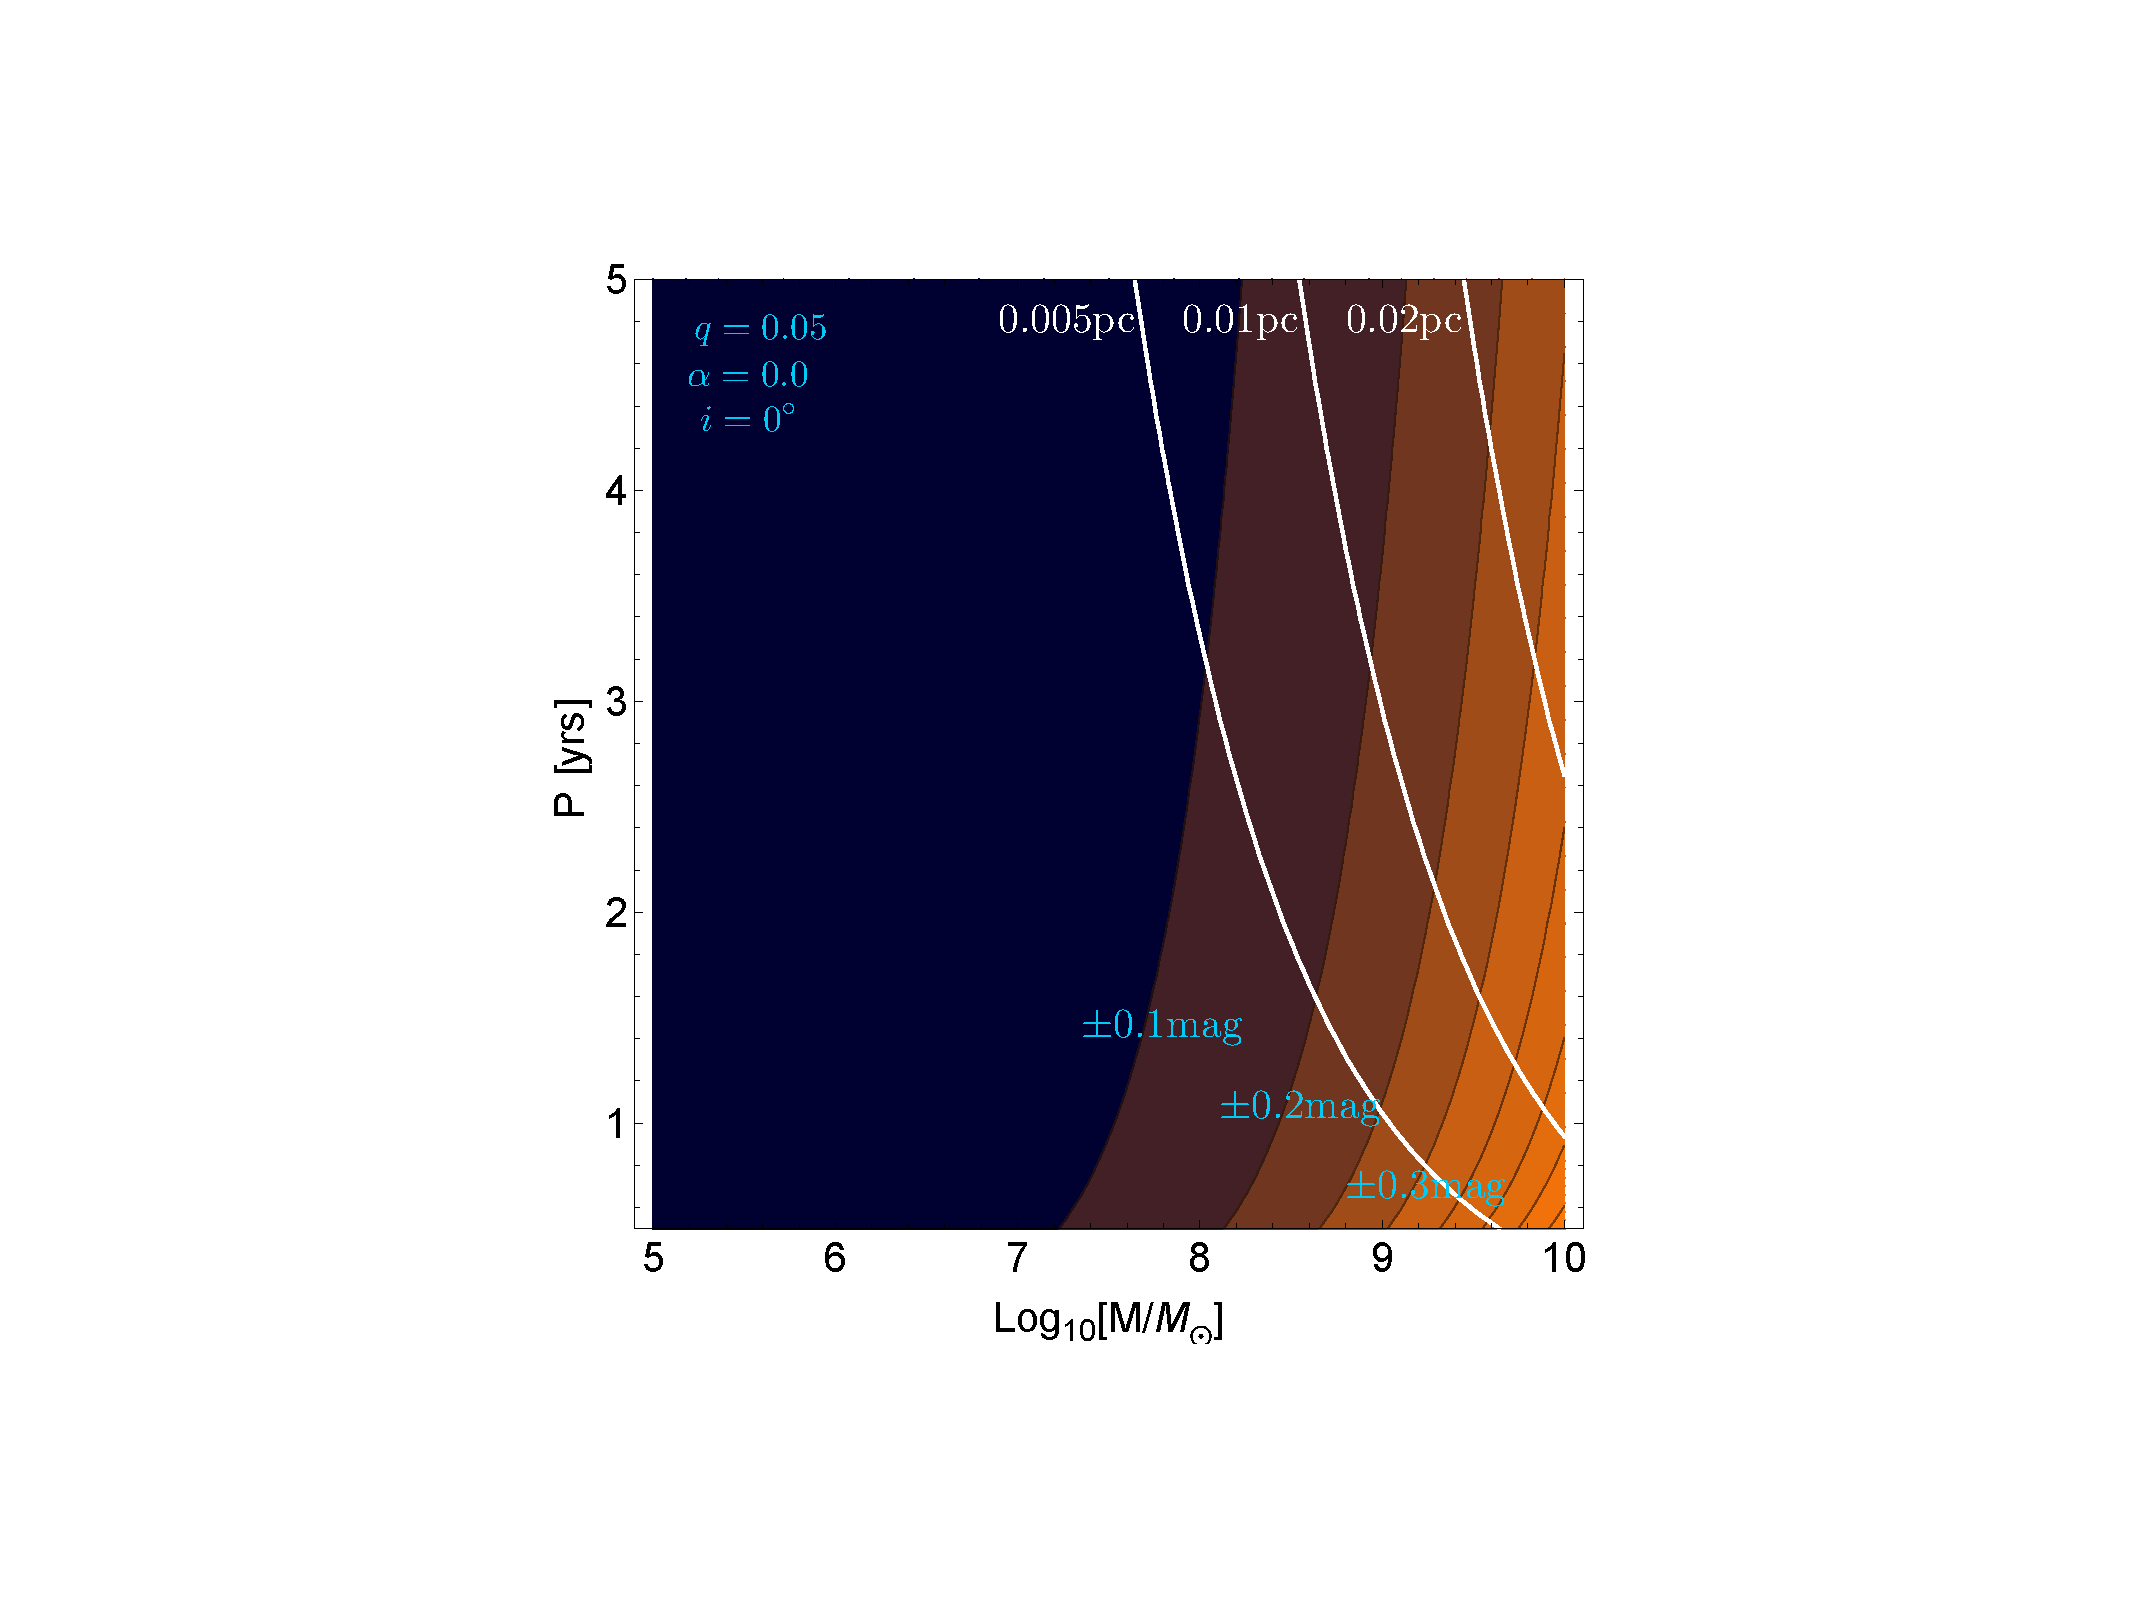
\includegraphics[scale=0.33]{figures/ch5/boosting_Pbin_M.pdf} \hspace{20pt} 
%
\end{array}$
\end{center}
\caption{Representative binary total masses and orbital periods for which Doppler boosting is an important cause of periodicity. White contours are binary separations at the given orbital period and binary mass. Cyan contours estimate the ratio of the light crossing time at the inner edge of a dust distribution $t_d$ (see \S \ref{S:PDs}) to the binary orbital period. We have assumed a mass ratio of $q=0.05$, an edge-on viewing of the binary ($I=0.0$ rad), and a spectral index $\alpha=0.0$.}
\label{Fig:boostParams}
\end{figure}
%%%%%%%%%%%%%%%%%%%%%%%%%%%%%%%%%%%%%%%%%%%%%%%%


\subsection{System Scales} 
The important system size scales are the binary separation and the inner edge of the
dust distribution. The binary separation is given by the total binary mass $M$
and orbital period $P$
\begin{equation}
a = \left(\frac{P}{2 \pi} \sqrt{GM} \right)^{2/3}.
\label{Eq:Bsep}
\end{equation}
The inner edge of the dusty torus is set by the onset of dust sublimation. 
For a source with luminosity $L = \epsilon L_{\rm{Edd}}(M)$, dust sublimates at radii
\begin{equation}
\Rin \lsim 0.9 \epsilon^{1/2}_{0.1} \left(\frac{M}{10^9 \Msun }\right)^{1/2}  \left(\frac{1800 K}{ T_{\rm{sub}} }\right)^{2.6} \rm{pc},
\label{Eq:Rd}
\end{equation}
where $\epsilon_{0.1} \equiv 0.1$ assumes that the total binary luminosity is
one tenth of the Eddington rate, and we assume that the inner, hottest region
of the dust torus is composed of graphites which sublimate at temperature
$T_{\rm{sub}} \sim 1800 K$ \citep{MorTrakhtenbrot:2011, MorNetzer:2012}. $R_d$
is the inner edge of the dusty torus, which we treat as a free parameter in
our model but interpret in the context of Eq. (\ref{Eq:Rd}). 




\section{Model Derivation}
\label{S:Derivation}
\subsection{Isotropic Emission From a Central Source}
\label{S:FISOderivation}

The novel addition to dust reverberation modeling that we put forth in this
work is the addition of a time-dependent anisotropic central source. To
compare to the case of an isotropic source and to aid in the build up to 
more complicated dust structures (forthcoming work), we first consider
an isotropic, time-dependent central source of continuum emission from an
infinitely thin dust shell. We assume for illustrative purposes that the dust
is optically thick to the UV/optical continuum source radiation and optically
thin to the reprocessed dust emission, in this way we can first explore the
dependence on dust geometry, and light travel time effects.

\subsubsection{Spherical Dust Shell}

We first assume the source with bolometric luminosity $L^{\rm iso}(t)$ to be
surrounded by an infinitely thin sphere of dust with radius $\Rin$. We adopt spherical
coordinates centered on the dust shell ($r,\theta,\phi$), with the observer
situated at coordinates $(r,  \theta, \phi) = (d, \pi/2, 0)$. The specific
flux at the dust shell is
\begin{equation}
F^{\rm iso}_{\nu} = \frac{L^{\rm iso}_{\nu}}{4 \pi R^2_d}.
\end{equation}
This flux of continuum radiation heats the surrounding dust. By assuming that
the dust is in radiative equilibrium with the heating source, and given an
efficiency of absorption/emission by the dust $Q_{\nu}$, we find the dust
temperature as a function of time by equating the power absorbed by a dust
grain to that radiated,
\begin{eqnarray}
\pi a^2_{\eff}\bar{Q}^{\rm src}_{\nu} F^{\rm iso}(t) = 4\pi a^2_{\rm eff} \int^{\infty}_{0}{Q_{\nu} \pi B_{\nu}\left[T_d(t)\right] \ d \nu } ,
\label{Eq:TdISO}
\end{eqnarray}
where $a_{\rm eff}$ is the effective grain radius and we assume that the same
$a_{\eff}$ describes the dust cross section for absorption as well as the
surface area for emission, $Q_{\nu}$ is the absorption/emission efficiency of
the dust, $\pi B_{\nu}$ is the blackbody flux from a uniformly emitting dust
grain at temperature $T^{\rm iso}_d$, and $\bar{Q}^{\rm src}_{\nu}$ denotes an
average over the source spectrum.

Radiation with wavelength $\lambda = c/\nu \lsim 2 \pi a_{\eff}$ will be
absorbed efficiently by dust grains. For longer wavelength radiation, grains of
the same size become transparent.  Hence for the absorption/emission
efficiency we choose $Q_{\nu}=1$ for frequencies above a cutoff $\nu_0 \sim c
(2 \pi a_{\eff})^{-1}$ and a power law fall off in efficiency for lower
frequency (long wavelength) radiation, $Q_{\nu} \equiv \rm{min}\left[
(\nu/\nu_0)^k, 1\right]$ where $k \geq 0$.\footnote{ For this form of
$Q_{\nu}$, the right hand side of Eq. (\ref{Eq:TdISO}) can be written in terms
of polylogarithmic functions.} We take fiducial values of $k=1$ and $c/\nu_0 =
1\mu$m such that our effective grain size is $a_{\eff} \sim 0.16 \mu$m,
consistent with the allowable range of hot Graphite grain sizes near the
sublimation radius \citep{LaorDraine:1993, MorNetzer:2012}. Because the
efficiency for absorption is unity for high frequency radiation, above $\sim$
$1\mu$m, we take $\bar{Q}^{\rm src}_{\nu} = 1$ throughout.


The observed flux due to one dust grain at temperature T is
\begin{eqnarray}
F^{\rm{grain}}_{\nu} &=& 2 \pi \int^{\theta_c}_0{ Q_{\nu} B_{\nu}(T) \cos{\theta_s} \sin{\theta_s} d \theta_s} = \left(\frac{ a_{\rm{eff}} }{d}\right)^2 Q_{\nu} \pi B_{\nu}(T) \\ \nonumber  
\theta_c &=& \sin^{-1}\left( \frac{ a_{\rm{eff}}}{d}\right) .
\end{eqnarray}
where $\theta_s = \theta_c$ is the angle subtended on the sky by a dust grain
with radius $ a_{\rm{eff}}$ at a distance $d$ from the observer. Given the
grain number density, the time dependent dust temperature everywhere in the
shell (Eq. (\ref{Eq:TdISO})), and assuming that dust is
optically thin to its own emission, we compute the total observed flux from
heated dust grains
\begin{eqnarray}
\label{Eq:FnuSS}
 F^{\rm SS}_{\nu}(t) &=& \left(\frac{ a_{\rm{eff}} }{d}\right)^2 \int^{2 \pi}_{0}{\int^{\pi}_{0}{ \Sigma_d Q_{\nu}  \pi B_{\nu}\left[T_d(t_{\em})\right]  R^2_d \sin{\theta} \ d \theta d\phi }}   \\ \nonumber 
 %
t_{\em}& =& t - \frac{\Rin}{c} \left( 1 - \sin{\theta} \cos{\phi}\right)  
\end{eqnarray}

where $\Sigma_d$ is the surface number density of the dust shell; $\Sigma_d
\rightarrow \pi^{-1} a^{-2}_{\eff}$ in the limit that all UV radiation is
absorbed by the sphere. The most important aspect of the above equation is
that we have evaluated the temperature at the time $t_{\em}$; if light leaving
the front of the dust shell reaches an observer at time $t$, then light
emitted from the location ($\Rin$, $\theta$, $\phi$) will reach the observer
at time $t_{\em}$. By integrating over all locations in the dust shell at time
$t$, we take into account the finite light travel time. Put another way, we
evaluate the time changing dust temperature at the retarded time. The left
panel of Figure \ref{Fig:Schm} illustrates this by drawing cross sections of
the paraboloids of constant light travel time (described by the equation for
$t_{\em}$). Conceptually, Figure \ref{Fig:Schm}, along with the definition of
$t_{\em}$, tells us that dust emission from a sphere of radius $R_d$, at time
$t$, is comprised of dust emission spanning a time interval of $2 \Rin /c$ in
the frame of the central emitting source. The lesson being that the
reprocessed dust emission will not necessarily be a phase shifted replica of
the continuum emission. We revisit the role of $t_{\em}$ in \S \ref{S:Interp:Sphere}.


The total observed flux at an instrument with bandpass function $W(\nu)$ is
 \begin{equation}
F_{W} = \int^{\infty}_{0}{  W(\nu) F_{\nu} d \nu  } \sim \int^{\nu_{\rm max}}_{\nu_{\rm min}}{ F_{\nu} d \nu}
\label{Eq:FISO}
 \end{equation}
where we assume that $W(\nu)$ is a top hat function with frequency
limits $\nu_{\rm min}$ and $\nu_{\rm max}$.



 %%%%%%%%%%%%%%%%%%%%%%%%%%%%%%%%%%%%%%%%%%%%%%%%
%%% FIGURE: Light Travel Geometry %%%
%%%%%%%%%%%%%%%%%%%%%%%%%%%%%%%%%%%%%%%%%%%%%%%%
\begin{figure}
\begin{center}$
\begin{array}{c c }
%
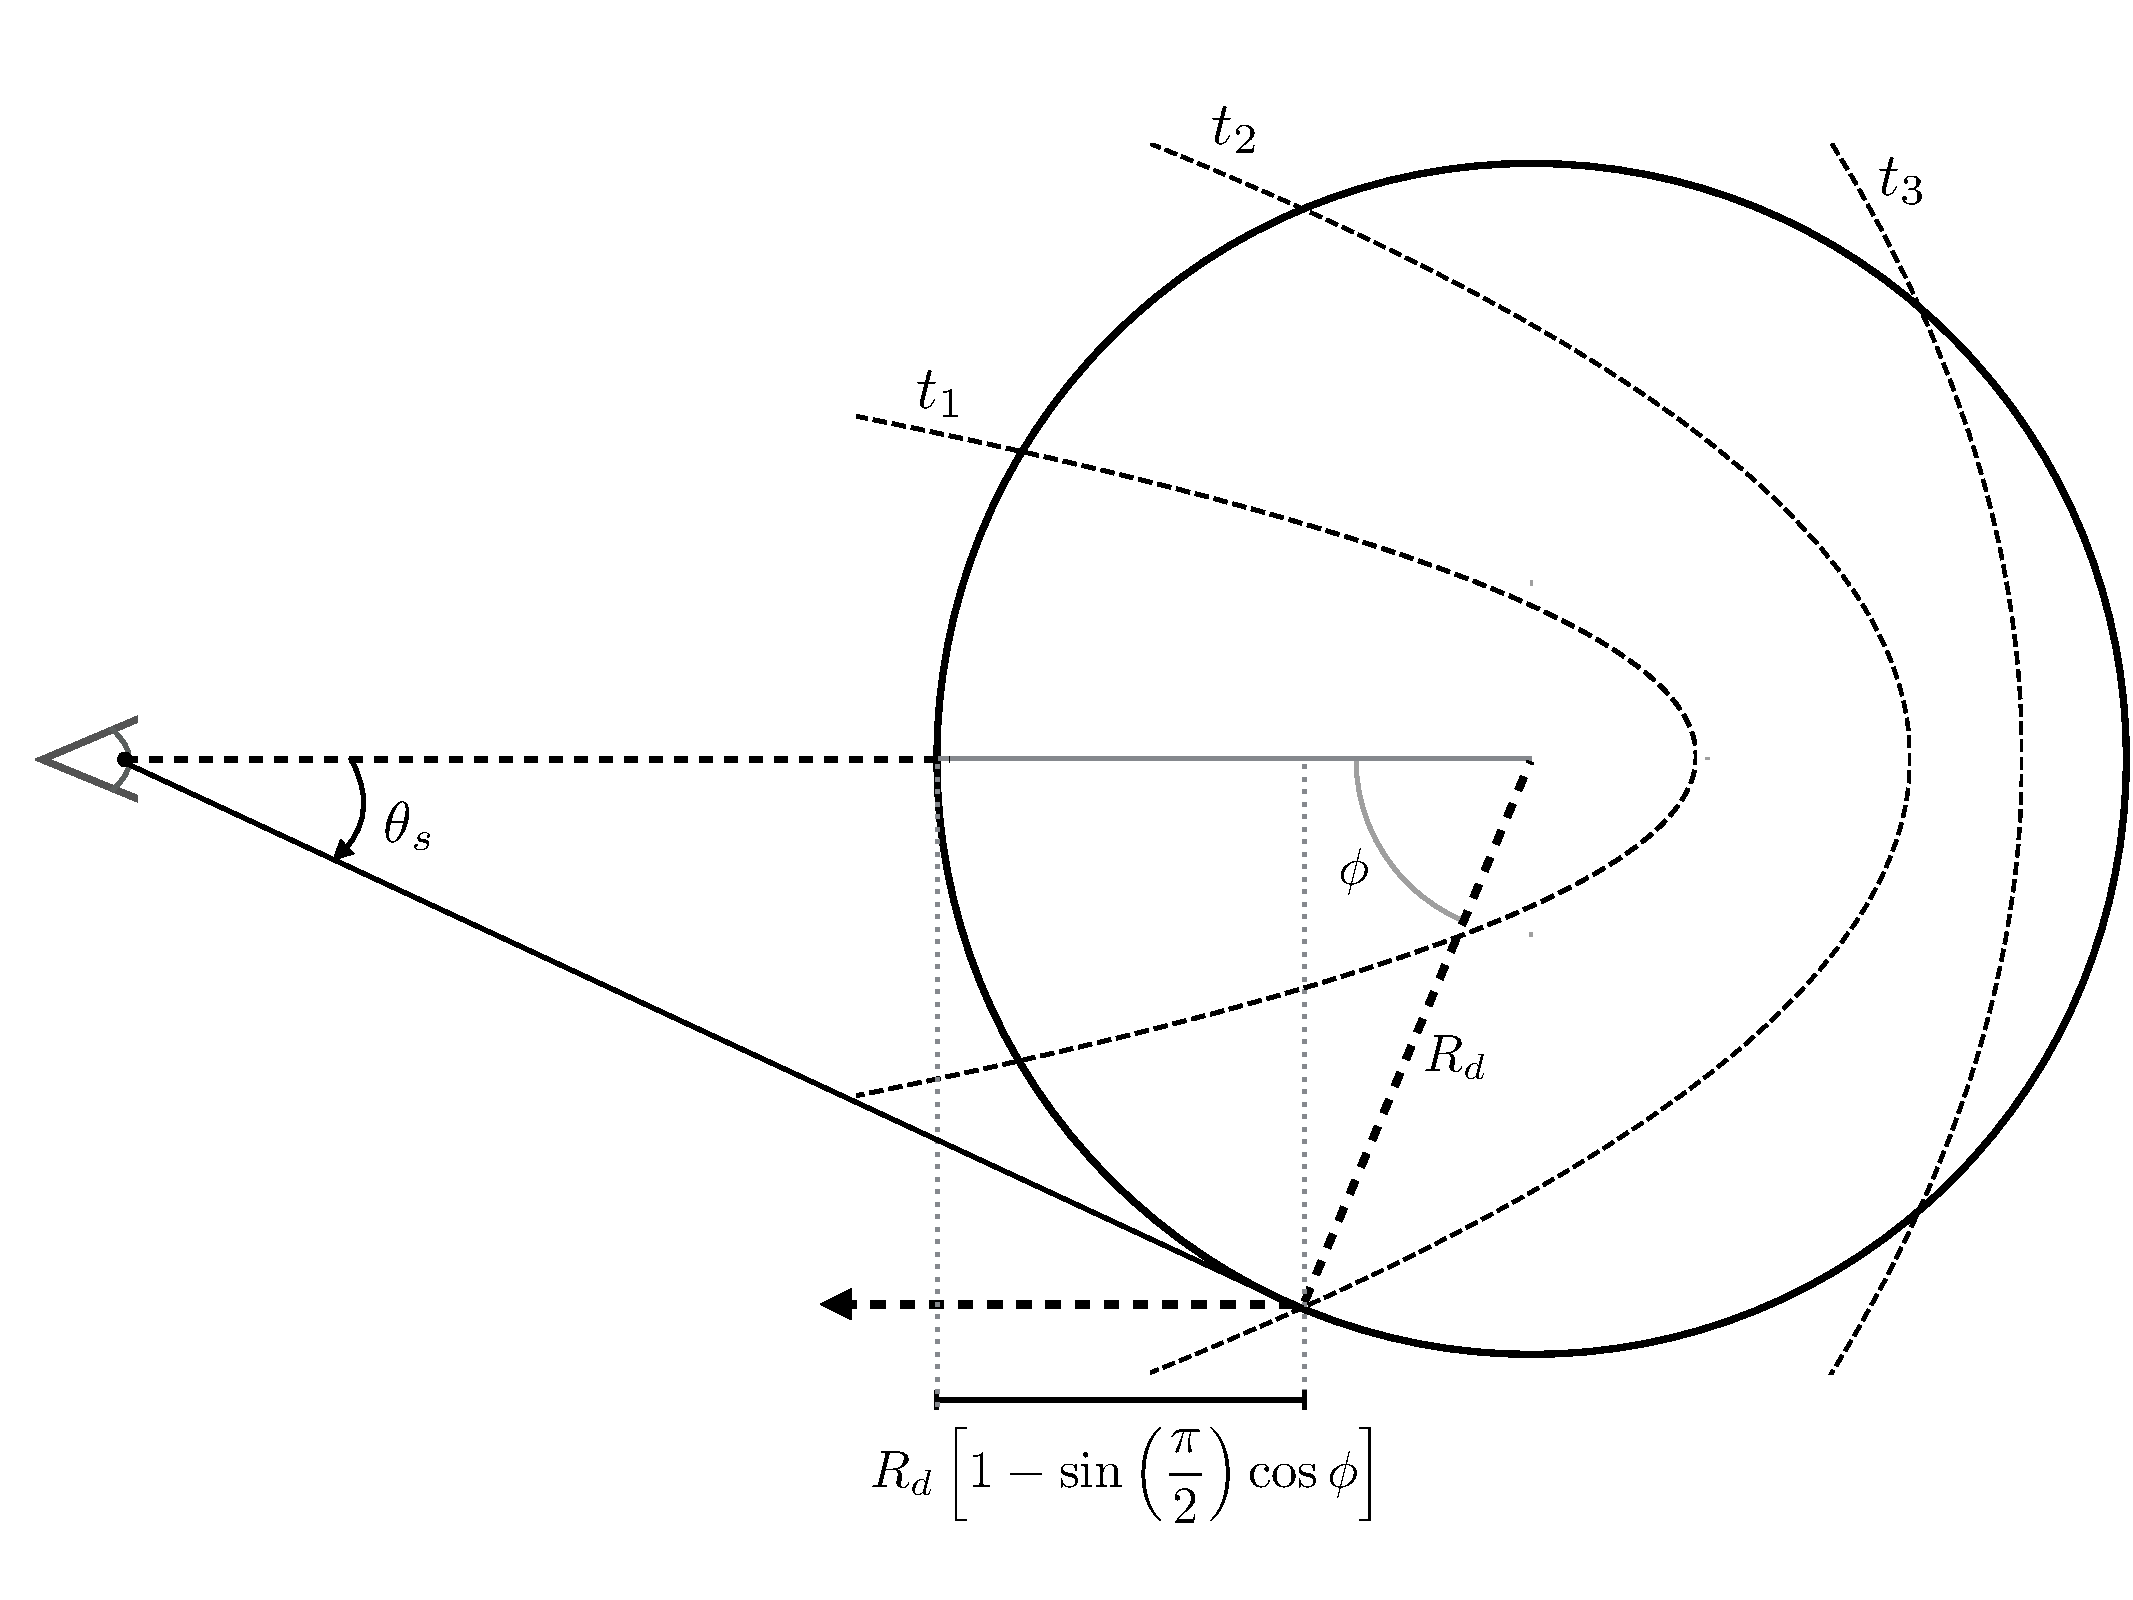
\includegraphics[scale=0.22]{figures/ch5/tem_schematic} \hspace{20pt} & 
 \includegraphics[scale=0.22]{figures/ch5/Torus_Schematic} 
%
\end{array}$
\end{center}
\caption{Left: light travel time geometry: The circle is a cross section of an emitting source. Light leaving the intersection of the emitting source and the parabola $t_1$ reaches the observer before light leaving the intersections of the source with $t_2$ and $t_3$. For a continuously emitting source, the observer's instantaneous view consists of light summed over all past parabolas intersecting the circle. Right: angles present in the torus geometry: $I$ is the inclination of binary orbital plane to observer's line of sight, $J$ is the inclination of torus axis to the plane perpendicular to the line of sight, $\theta_T$ is the opening angle of the torus, and $\theta$ is the polar spherical angle in our chosen coordinate system.}
\label{Fig:Schm}
\end{figure}
%%%%%%%%%%%%%%%%%%%%%%%%%%%%%%%%%%%%%%%%%%%%%%%%








%%%%%%%
\subsubsection{Torus Shell}
%%%%%%%

The dust sphere of the previous section has one geometric parameter, its
radius $R_d$. We expand upon the spherical model by cutting out portions of
the sphere to make an infinitely thin torus, or torus shell. This introduces a
second and a third dust geometry parameter: the opening angle of the torus
$\theta_T$ and the inclination of the torus to the line of sight $J$. These
angles and the binary inclination angle are drawn schematically (for a torus
with finite radial extent) in the right panel of Figure \ref{Fig:Schm}. For
the torus model we simply set the temperature found in Eq. (\ref{Eq:TdISO}) to
zero for
\begin{eqnarray}
\theta'(J) < \theta_T \quad \rm{or} \quad \theta'(J) > \pi - \theta_T
\end{eqnarray}
where $\theta'(J)$ is the polar coordinate in a coordinate system rotated
around the y axis by angle $J$.










%%%%%%% 
\subsection{Non-Isotropic, Doppler Boosted Emission - The Lighthouse} 
%%%%%%% 
To include the effects of Doppler boosting in the IR light
curve we only need to change the form of the source (UV/optical) flux. We assume that dust surrounds a
binary with total mass $M$ and separation $a$. Due to relativistic Doppler
boosting of a steadily emitting source attached to the secondary, the specific
flux received in the frame of the stationary dust shell differs from the
specific flux in the rest frame of the secondary BH as dictated by Eq.
(\ref{Eq:Dop1}). Assuming a rest frame flux $F^0_{\nu} \propto
\nu^{\alpha_{\nu}}$, the flux at the location of the dust shell is,
\begin{eqnarray}
F_{\nu}(t, \Rin, \theta, \phi) &=& \left[D(t, \theta, \phi)\right]^{3-\alpha_{\nu}} F^0_{\nu}(\Rin)  \nonumber \\
&=&  \left[D(t, \theta, \phi)\right]^{3-\alpha_{\nu}} \frac{L^0_{\nu}}{4 \pi r^2_2}  \\ \nonumber
D(t, \theta, \phi) &\equiv& \left[ \gamma \left(1 - \frac{v_{||}}{c} \right) \right]^{-1},
\label{Eq:DopFlux}
\end{eqnarray}
where $L^0_{\nu}$ is the rest frame, specific luminosity of the source,
$\gamma = \left[ 1 - (v_s/c)^2 \right]^{-1/2}$ is the Lorentz factor of the
secondary which orbits at speed $v_s = (1+q)^{-1}\sqrt{GM/a}$, $I$ is the
inclination angle of the binary's orbit to the line of sight, $\Omega$ is the
angular frequency of the binary and we assume throughout that the binary is on
a circular orbit. We continue to use the spherical coordinates as above with
($r,\theta, \phi$) centered on the binary center of mass and with the observer
situated at ($d,\pi/2$,0). We have approximated the distance from the
secondary to the dust shell as $\Rin$ (see Eq. \ref{Eq:aORd} below).

The line of sight velocity $v_{||}$ in the Doppler factor $D$ is the line of
sight speed of the secondary BH as  observed by a dust grain at position
$\mathbf{\hat{r}}_{\rm{dust}}$ in the dust shell. Written in terms of
barycentric coordinates $(r,\theta, \phi)$,
\begin{eqnarray}
\frac{v_{||}}{c} &=& \frac{\mathbf{v_{s}} \cdot \mathbf{\hat{r}}_{\rm{dust}} }{c}\\ \nonumber 
& = & \beta  \left[ \cos{I} \cos{(\phi_0+\Omega t)} \sin{\theta}\cos{\phi} - \sin{(\phi_0+\Omega t)} \sin{\theta}\sin{\phi} - \sin{I} \cos{(\phi_0+\Omega t)} \cos{\theta}  \right],
\label{Eq:vlos}
\end{eqnarray}
where $\phi_0$ is the $\phi$ coordinate of the secondary at $t=0$ and we have
parameterized the secondary orbital velocity as $\beta \equiv a (1+q)^{-1}
\Omega$ which depends on the binary mass ratio $q$, total mass $M$, and period
$P$ through the binary orbital frequency $\Omega$ and separation $a$ (Eq. \ref{Eq:Bsep}).



Just as for the isotropically emitting source, we determine the temperature of
each patch of the dust shell, by assuming radiative equilibrium between the
incident UV/optical flux and the dust. The difference here is that the incident flux and resulting dust
temperature are now spatially varying across the sphere. The analogue of Eq.
(\ref{Eq:TdISO}) becomes
\begin{equation}
\label{Eq:TdDop1}
\bar{Q}_{\nu} \int^{\infty}_{0}{F_{\nu}(t, \theta, \phi)  \ d \nu } =   4 \int^{\infty}_{0}{Q_{\nu} \pi B_{\nu}\left[T_d(t,\theta, \phi)\right] \ d\nu}.
\end{equation}
We approximate the LHS of the above equation as
\begin{equation}
\label{Eq:TdDop}
\left[D(t, \theta, \phi)\right]^{3-\bar{\alpha}} \frac{L^0}{4 \pi R^2_d}  =   4 \int^{\infty}_{0}{Q_{\nu} \pi B_{\nu}\left[T_d(t,\theta, \phi)\right] \ d\nu}. 
\end{equation}
where $L^0$ is the bolometric source luminosity and we have approximated the
frequency dependent source spectra slope $\alpha_{\nu}$ by an average
$\bar{\alpha}$ over source frequency. This solution for the dust temperature
can be used in either of the solutions for $F_{\nu}$ derived for an isotropic
source in \S \ref{S:FISOderivation}.










\section{Results}
\label{S:PDs}

We now identify the effect of the model parameters on the IR light curves. For
our purposes, the most important features of the reverberated light curve are
the average brightness, phase, and variability amplitude relative to the
UV/optical continuum.







\subsection{Sphere} 
\label{S:Interp:Sphere} 

For demonstrative reasons, we first consider the simplest case: isotropic,
sinusoidal emission by the central source, and ignoring light travel time
effects as well as dust absorption/emission efficiency ($Q_{\nu} \rightarrow
1$). In this case, the dust temperature is observed to be constant across the
dust sphere at a given time,
\begin{equation}
T^4_d(t) =  \frac{L(t)}{16 \pi R^2_d \sigma},
\end{equation}
where $L(t)$ is the time variable continuum (UV/optical) emission from 
the central illuminating source, and $\sigma$
is the Stephan-Boltzmann constant. The IR luminosity of one grain is simply $4
\pi a^2_{\eff} \sigma T^4_d$ and the total IR luminosity is found by
multiplying by the number of grains, $\Sigma_d 4 \pi R^2_d$, then
\begin{equation}
L_{\rm{IR}} =  \Sigma_d \pi a^2_{\eff} L \rightarrow L
\end{equation}
where the $\rightarrow$ holds in the limit that  $\tau  \rightarrow 1$  so
that $\Sigma_d \rightarrow \pi^{-1} a^{-2}_{\eff}$. When light travel time is
ignored, the IR light curves should track exactly the UV light curves; we
confirm this to be the case in our numerical scheme for solving the equations
of \S \ref{S:Derivation} by setting $\nu_0 = 1$ and $t_{\em} = t$ and finding
agreement of IR and UV/optical light curves.


Re-introducing the time delay, the assumption that $T_d(t)$ is constant across the sphere breaks down,
\begin{equation}
T^4_d(t, \theta, \phi) =  \frac{L\left( t_{\em}(t, \theta, \phi) \right)}{16 \pi R^2_d \sigma},
\end{equation}
and the IR luminosity, integrated over all frequencies, becomes
\begin{eqnarray}
L_{\rm{IR}} 
&=&\Sigma_d 4 \pi a^2_{\eff} \int^{2 \pi}_0{\int^{\pi}_0{  \frac{L\left( t_{\em}(t, \theta, \phi) \right)}{16 \pi R^2_d } R^2_d \sin{\theta} d\theta d\phi }} \nonumber \\
&=&  \Sigma_d \pi  a^2_{\eff} L^0  \left[ 
  1 +  A \rm{sinc}{\left( \Omega t_d \right)}  \sin{ \left( \Omega \left( t - t_d \right) \right)  }
   \right],
   \label{Eq:LIR_sp}
\end{eqnarray}
for which the last line follows only if we rotate our coordinate system so that the observer is looking down the z-axis, instead of the x-axis (or equivalently if $J= \pi/2$). Here $\rm{sinc}(x) = \sin{x}/x$ is the cardinal sine function,
and we assumed that the UV/optical luminosity is
\begin{equation}
L(t) =  L^0  \left[ 
  1 +  A \  \sin{ \left( \Omega t  \right)  }
   \right].
\end{equation}
with average luminosity $L^0$ and amplitude of modulation $A$.

From this simple expression we can learn a great deal about reverberated IR emission in general.
First, we find, as expected, that the average luminosity of the UV/optical emission, in the
case where the dust is optically thick to continuum emission, is the same as the average luminosity of the IR. Also as
expected, we find that the IR is modulated at the same period as the UV, but
with a phase lag given by the light travel time from the central source to the
dust shell. What we find that is new, is that the amplitude of modulation is
necessarily diminished by a factor,
\begin{eqnarray}
\frac{A_{\rm{IR}}}{A} = \frac{1}{2 \pi}\frac{P}{t_d} \sin{\left[ 2 \pi\frac{t_d}{P} \right]},
\label{Eq:AIRoAUV}
\end{eqnarray}
where $A_{\rm{IR}}$ is the amplitude of IR modulation, $A$ is the amplitude of
UV/optical modulation, we have defined $t_d \equiv R_d/c$, and $P = 2 \pi
/\Omega$, the period of the varying source. 

Eq. (\ref{Eq:AIRoAUV}) tells us that the amplitude of IR modulation is
determined purely by the ratio $t_d/P$. For $t_d/P \rightarrow 0$ the IR
amplitude matches the UV amplitude. As $t_d/P$ increases, the relative IR to
UV/optical amplitude decreases, falling to  zero amplitude at $t_d/P  \gg 1$
and at the values where $t_d/P = \frac{m}{2}$. This analytic result Eq.
(\ref{Eq:LIR_sp}) is depicted in Figure \ref{Fig:AIRoAUV_sp}, along with the
results of our numerical calculation of the corresponding expressions in \S
\ref{S:Derivation}. In the limit that we integrate over all frequencies, We
find good agreement between analytic and numerical results.




The reason for a decreased IR magnitude can be understood in the zeros of Eq.
(\ref{Eq:AIRoAUV}). When $t_d$ is an integer multiple of half the variability
period, the IR variability drops to zero. This is because, at time $t_0$, the
dust temperature ranges from $T(t_0)$ at the front of the sphere to $T(t_0 -
2t_d)$ at the back of the sphere. The spatial variation of the brightness
across the sphere is sinusoidal along the line of sight, weighted by the size
of the emitting region, smallest at the sphere front and back, largest in the
center. When $t_d/P = \frac{m}{2}$, the spatial variation of dust emission spans
an integer number of whole variability cycles. Hence, integrating over the sphere
gives the average luminosity at all times, with no variation. 

When $t_d/P \neq \frac{m}{2}$, a non integer fraction of the entire cycle is
observed at once. Looking down the z-axis of the sphere, each $x-y$ cross
section will have a different temperature. As the non-integer fraction of a
variation period sweeps through the sphere, uncanceled by its counterpart in
the missing part of a full period, it lights up larger and smaller $x-y$
circles causing the observed IR variability.  The change in sign of
$A_{\rm{IR}}/A$ in Figure \ref{Fig:AIRoAUV_sp} is a $\pi$ phase change in the
IR light curve reflecting whether the variability causing deficit is brighter
or dimmer than the average (a dim spot at the closest and furthest points of
the sphere corresponds to a peak of the light curve, a hot spot in the same
place corresponds to a trough).



%%%%%%%%%%%%%%%%%%%%%%%%%%%%%%%%%%%%%%%%%%%%%%%%
%%% FIGURE: Sphere amplitude ISO vs Dop%%%
%%%%%%%%%%%%%%%%%%%%%%%%%%%%%%%%%%%%%%%%%%%%%%%%
\begin{figure}
\begin{center}
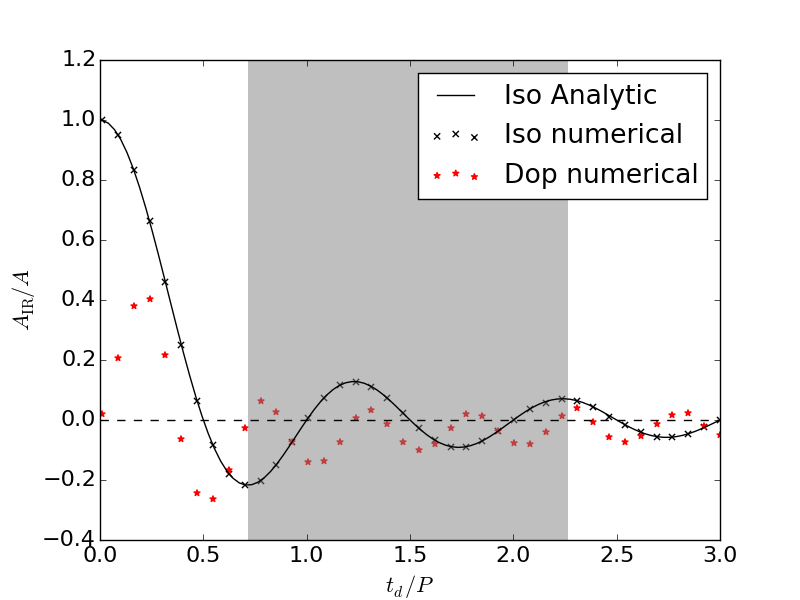
\includegraphics[scale=0.33]{figures/ch5/AIRplots/DopvsISO_AIRoAUV_J1p5708_numin0_numx5_reclim2_TRHS}
\end{center}
%
\caption{The amplitude of IR variability $A_{\rm{IR}}$ in terms  of the
UV/optical amplitude $A$ for a spherical dust shell which absorbs all of the
UV/optical radiation and emits it all in IR. The IR amplitude is given by the
absolute value of the plotted quantity while positive and negative values
denote a half cycle phase difference. Numerical values are presented for both
isotropic (black x's) and Doppler (red stars) sources. They are computed from
the peaks and troughs of solutions for IR light curves laid out in \S
\ref{S:Derivation}. The analytic solution (solid line) is Eq. \ref{Eq:LIR_sp}.
The shaded region contains typical values of $t_d/P$ computed for the MBHB
candidate PG 1302.}
%
\label{Fig:AIRoAUV_sp}
\end{figure}
%%%%%%%%%%%%%%%%%%%%%%%%%%%%%%%%%%%%%%%%%%%%%%%%



Figure \ref{Fig:AIRoAUV_sp} also plots the numerical result for the Doppler
boosted source. The amplitude of modulations for the Doppler case falls to
zero for $t_d/P \rightarrow 0$ where as, in the same limit of the isotropic
case, the IR modulation increases in amplitude to match the UV amplitude. The
difference comes in the nature of the variation between the two cases. Because
the Doppler boosted emission is observer dependent, and coming from a steady
rest-frame source, conservation of energy requires that the total emission
integrated over a sphere will not vary in time (even though an observer at
each point on the sphere sees a varying flux). Observed IR variability arises
because finite light travel times from each part of the sphere cause the
observer to see each cross section, in the plane perpendicular to the
observer, heated at different times in the source evolution (see Figure
\ref{Fig:Schm}), this changes as the rotating lighthouse pattern of the
Doppler boosted source varies from front to back of the dust sphere. As $t_d/P
\rightarrow 0$, the time delay becomes insignificant and the observed IR
amplitude falls to zero.



%zeros of Doppler curve

Figure \ref{Fig:AIRoAUV_sp} shows that the Doppler IR emission has zero
variability amplitude at values of $t_d/P$ which are offset from the analogous
nodes of the isotropic case. This is due to the anisotropic nature of the
Doppler emission. The distribution of observed temperatures across the dust
sphere in the isotropic case is simply a sinusoid along the line of sight. In
the Doppler case however, a (asymmetric) dipole temperature pattern is
imprinted on the dust shell in the frame of the emitting source
(\textit{e.g.}, not taking into account light travel time to an observer).
This dipole pattern sweeps around with the binary like a lighthouse
illuminating the dust. Taking into account light travel time to an observer,
this dipole pattern gets smeared out along the direction of the observer's
line of sight (which, as mentioned above, is why any variability is observed
at all). The nodes of the Doppler IR amplitude in Figure \ref{Fig:AIRoAUV_sp}
occur when integration of the blended dipole pattern over the sphere gives a
time constant flux. This depends, as in the isotropic case, on the ratio of
dust light crossing time to source variability period.







%Absorption 
We have so far ignored the efficiency of dust absorption and emission
$Q_{\nu}$. Figure \ref{Fig:Qvon} shows that in the case so far, where we
integrate over all frequencies, dust absorption/emission does not affect our
result. In Figure \ref{Fig:Qvon}, the analytic solution Eq. (\ref{Eq:LIR_sp})
(solid line) matches the over-plotted x's, which are the result of
numerical integration including absorption/emission efficiencies.



When integrating over a specific wave band, however, the variation in dust
temperature will shift the dust spectrum blue-ward and red-ward over time.
This will cause an extra source of instrument dependent IR variability not
considered so far. This band specific variability will depend on the
absorption/emission efficiency of the dust, and specifically where the cutoff
in efficiency occurs relative to the observing band. A procedure designed to
fit to data should take the dust parameters $\nu_0$ and $k$ of the efficiency
function $Q_{\nu} = \rm{min}\left[ \left( \nu/ \nu_0 \right)^{k}, 1\right]$
into account.








%%%%%%%%%%%%%%%%%%%%%%%%%%%%%%%%%%%%%%%%%%%%%%%%
%%% FIGURE: AIR with Dust eff%%%
%%%%%%%%%%%%%%%%%%%%%%%%%%%%%%%%%%%%%%%%%%%%%%%%
\begin{figure}
\begin{center}$
\begin{array}{c}
%FISO and DOP 
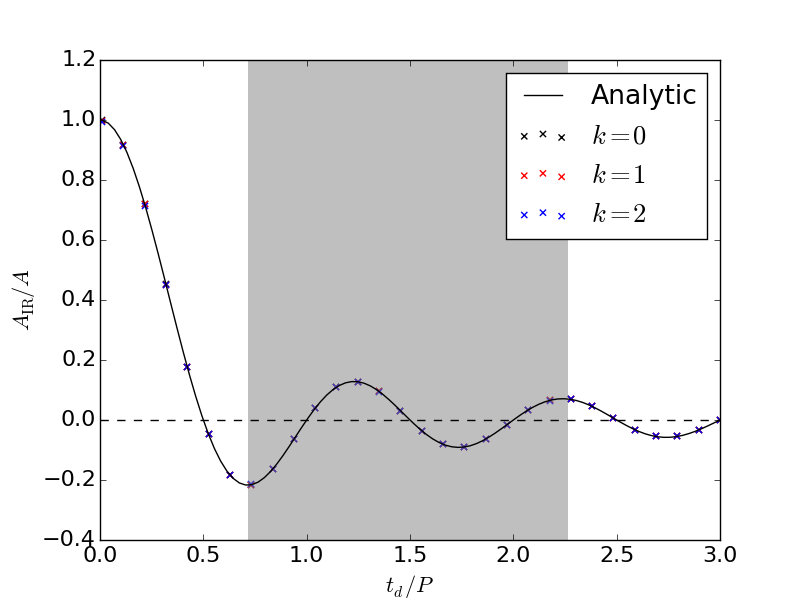
\includegraphics[scale=0.33]{figures/ch5/AIRplots/Qv_vark__AIRoAUV_J1p5708_numin0_numx5_reclim2_TRHS}  
%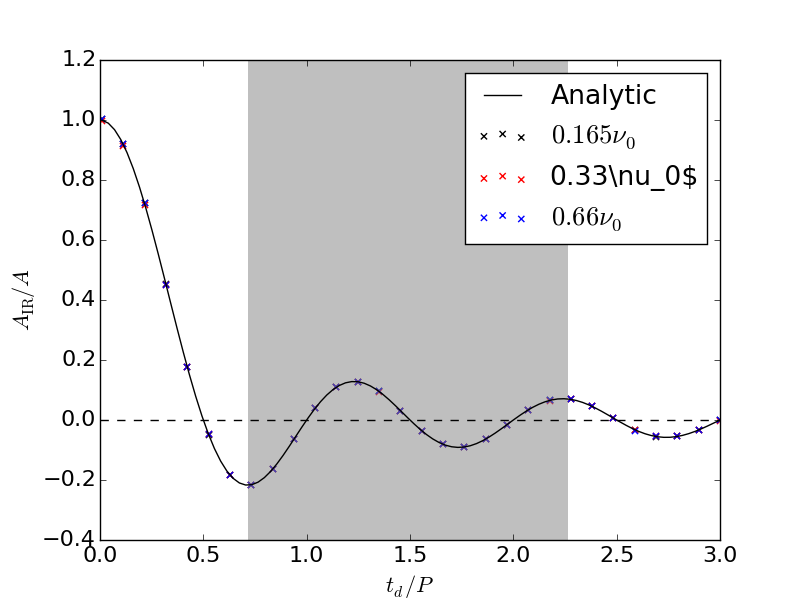
\includegraphics[scale=0.3]{figures/ch5/AIRplots/Qv_varnu0_AIRoAUV_J1p5708_numin0_numx5_reclim2_TRHS} 
\end{array}$
\end{center}
\caption{The same as Figure \ref{Fig:AIRoAUV_sp} except showing that, when integrating over all frequencies, the dust absorption/emission efficiency $Q_{\nu} = \rm{min}\left[ \left( \nu/ \nu_0 \right)^{k}, 1\right]$ does not affect the IR variability amplitude. Varying $\nu_0$ also has no effect on the relative amplitude. In the case of a finite wave band, however, the choice of $Q_{\nu}$ will be relevant.}
\label{Fig:Qvon}
\end{figure}
%%%%%%%%%%%%%%%%%%%%%%%%%%%%%%%%%%%%%%%%%%%%%%%%





Numerically evaluating the expressions of \S \ref{S:Derivation}, We plot the
UV/optical (source) and IR (reverberated) light curves for the spherical case
in Figure \ref{Fig:SphDopvISO}. The left panel of Figure \ref{Fig:SphDopvISO}
assumes an isotropic source and the right panel assumes a Doppler boosted
source. We include the dust absorption/emission efficiency and integrate over
all frequencies. The model parameters and their fiducial values are given in
Table \ref{Table:params}.

The IR amplitudes of the light curves in Figure \ref{Fig:SphDopvISO} are in
agreement with the predictions from Figure \ref{Fig:AIRoAUV_sp}. Each IR light
curve is for a dust sphere at radius given by a multiple of $R_0 = 0.9$pc as
labeled in the Figure legend. For the choice of $\Omega = 2\pi c/R_0$ this
gives $t_d/P = 0.8$ for the yellow curve, $t_d/P = 1$ for the red curve, and
$t_d/P = 1.\bar{33}$ for the brown curve. Comparing \ref{Fig:AIRoAUV_sp} and
\ref{Fig:SphDopvISO}, we find agreement.

For the isotropic case we confirm the the IR light curves lag the UV/optical
continuum by the fraction $t_d/P$ of a cycle. It is important to note that for
$A_{\rm{IR}}/A$ of different signs, the corresponding light curves are half a
cycle out of phase. This means that the yellow curve, for which $A_{\rm{IR}}/A
< 0$ is $0.5 + 0.8$ cycles behind the UV/optical (shifted to the right in
Figure \ref{Fig:SphDopvISO}), while the brown curve, for which $A_{\rm{IR}}/A
> 0$, is $1.\bar{33}$ cycles behind. This half cycle phase shift would be
important to recognize if attempting to determine the size of a dusty region
from IR phase lags of a sinusoidally varying source.

Importantly, for the Doppler case, comparison of the left and right panels of
Figure \ref{Fig:SphDopvISO} shows that the IR phase lag is offset from the
isotropic phase lag. It does, however, appear to be set by $t_d/P$ alone, as
computation of the same light curves for different $P$ and $t_d$ but the same
$t_d/P$ give the same IR lightcurves. If we were not integrating over all
frequencies this would not be the case because $R_d$ sets $t_d$ and also the
average dust temperature, which sets the spectrum of IR emission.





%%%%%%%%%%%%%%%%%%%%%%%%%%%%%%%%%%%%%%%%%%%%%%%%
%%% FIGURE: Sphere IR light curves ISO vs Dop%%%
%%%%%%%%%%%%%%%%%%%%%%%%%%%%%%%%%%%%%%%%%%%%%%%%
\begin{figure}
\begin{center}$
\begin{array}{c c c}
%FISO and DOP  vary Rin
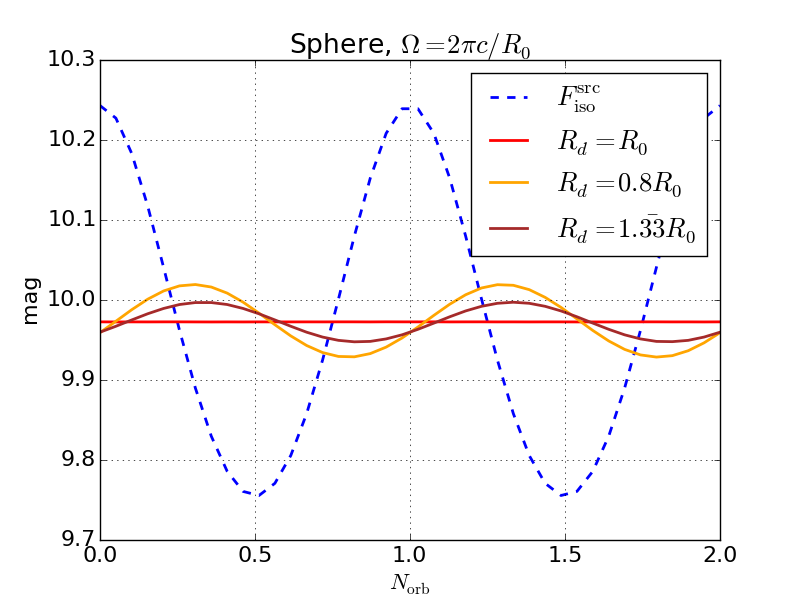
\includegraphics[scale=0.33]{figures/ch5/Sphere/FISO_Sphere_nrm0_Om1_VaryRin_numin0_numx10} & 
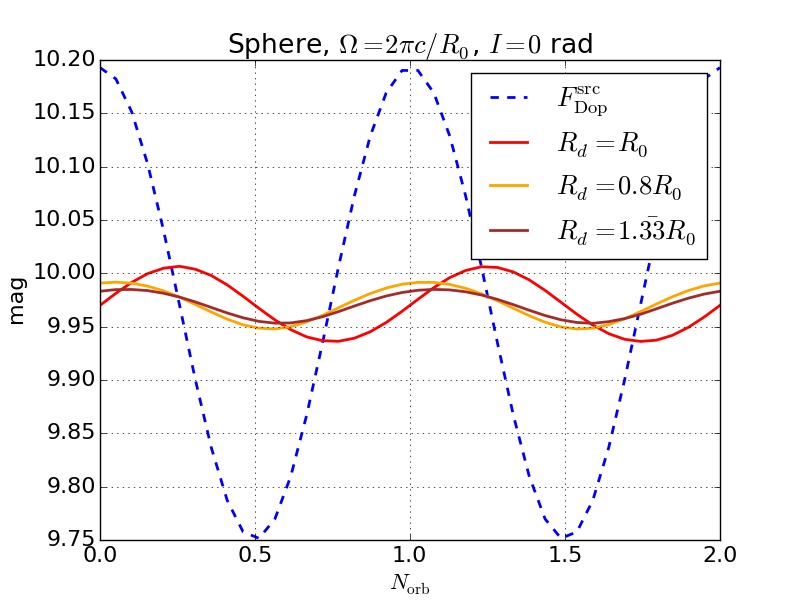
\includegraphics[scale=0.33]{figures/ch5/Sphere/FDop_1R0_Sphere_nrm0__J0_Inc0_VaryRin_numin0_numx10} &
%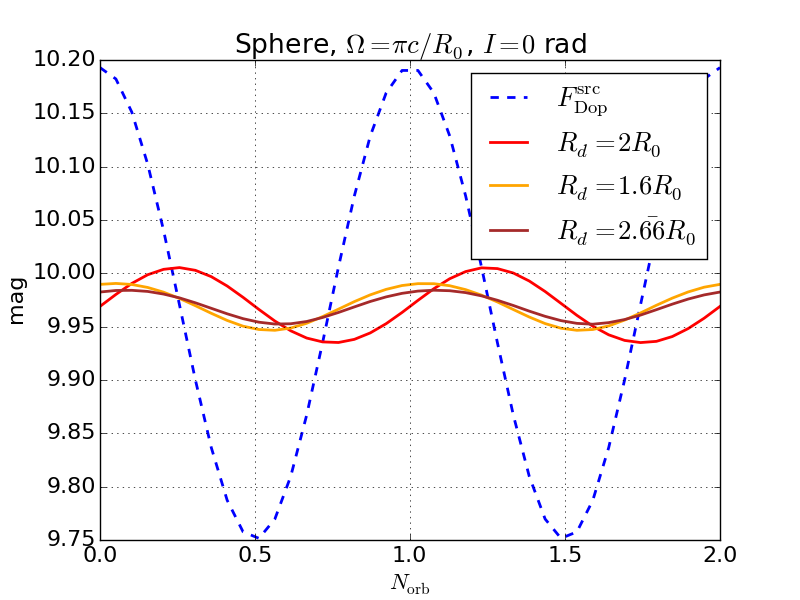
\includegraphics[scale=0.27]{figures/ch5/Sphere/FDop_2R0_Sphere_nrm0__J0_Inc0_VaryRin_numin0_numx10}
\end{array}$
\end{center}
\caption{Spherical dust shell model. The solid lines are the IR light curves generated by reverberation of the UV/optical continuum (dashed blue line) from a spherical dust shell with radius $R_d$ (measured in units of $R_0$ see Table \ref{Table:params} for fiducial parameter values). The left panel is for an isotropic central source, and the right panel is for a Doppler boosted central source.}
\label{Fig:SphDopvISO}
\end{figure}
%%%%%%%%%%%%%%%%%%%%%%%%%%%%%%%%%%%%%%%%%%%%%%%%







Finally we demonstrate the dependence of binary inclination angle in the
Doppler case. As discussed above, the observed IR amplitude in the Doppler
case will drop to zero if there is no time variation in dust temperature from
front to back of the dust sphere. This occurs when the binary is at a face-on
inclination to the observer line of sight, and is illustrated in Figure
\ref{Fig:Sph_VarI}. Because the amount of back-to-front variation is dependent
only on the binary inclination in the spherical case, IR and UV/optical
amplitudes scale together, so that the the $A_{\rm IR}/A$ curve in Figure
\ref{Fig:AIRoAUV_sp} is independent of binary inclination. This will not be
the case for a torus dust geometry.

%%%%%%%%%%%%%%%%%%%%%%%%%%%%%%%%%%%%%%%%%%%%%%%%
%%% FIGURE: Sphere IR light curves ISO vs Dop%%%
%%%%%%%%%%%%%%%%%%%%%%%%%%%%%%%%%%%%%%%%%%%%%%%%
\begin{figure}
\begin{center}
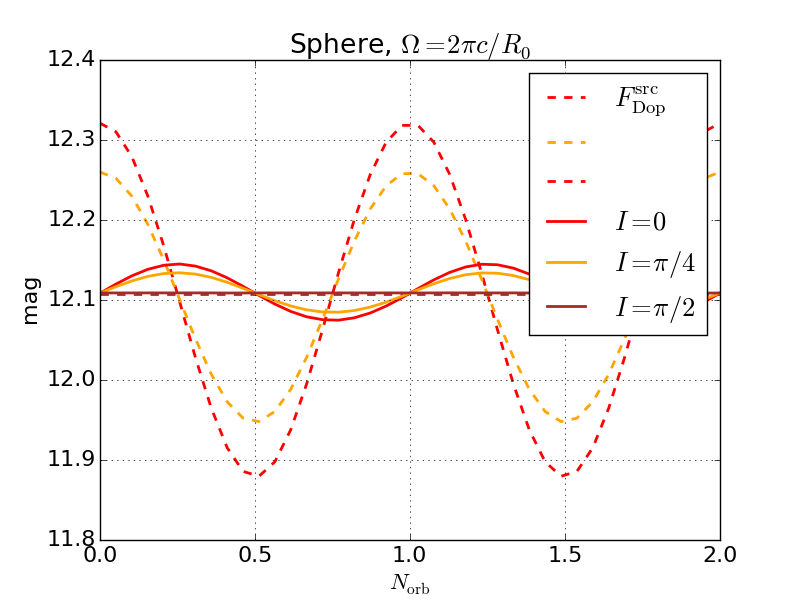
\includegraphics[scale=0.33]{figures/ch5/Sphere/FDop_Sphere_nrm2p13871_Rde2p73218e+18_VaryInc_numin0_numx10} 
\end{center}
\caption{The same as Figure \ref{Fig:SphDopvISO} but for multiple binary inclination angles and $R_d = R_0$.}
\label{Fig:Sph_VarI}
\end{figure}
%%%%%%%%%%%%%%%%%%%%%%%%%%%%%%%%%%%%%%%%%%%%%%%%






 
\subsection{Geometrically Thin Torus} 
\label{S:Interp:ThinTor}

The result from the previous section can be adapted to that of a torus with
infinitesimal radial extent, where regions of the sphere with $\theta \leq
\theta_T$ are removed, and the observer is looking down the axis of the torus
with ($J=\pi/2$: see Figure \ref{Fig:Schm}). We find,
\begin{equation}
L_{\rm{IR}} =  \Sigma_d \pi  a^2_{\eff} L^0  \cos{\theta_T} \left[ 
  1 +  A  \ \rm{sinc}{\left( \Omega t_d \cos{\theta_T}\right)}  \sin{ \left( \Omega \left( t - t_d \right) \right)  }
   \right].
   \label{Eq:LIR_thT}
\end{equation}
As expected, the total IR luminosity, and hence the total maximum variability
amplitude decreases proportionally to the covering factor of the torus.

The first panel in Figure \ref{Fig:AIRoAUV_tr} plots the relative IR to
UV/optical variability amplitude for different opening angles for an observer
looking down the axis of the opening. The analytic result Eq.
(\ref{Eq:LIR_thT}) (solid lines in Figure \ref{Fig:AIRoAUV_tr}) matches
the result of numerical evaluation of the calculation presented in \S
\ref{S:Derivation} (x's in Figure \ref{Fig:AIRoAUV_tr}). The middle and
right panels of Figure \ref{Fig:AIRoAUV_tr} extend upon the analytic result by
rotating the torus by angles $J=\pi/4$ and $J=0$.

The effect of changing the torus opening angle $\theta_T$ is two fold, it
decreases the total IR luminosity, and hence the IR amplitude of variability
compared to the UV amplitude. It also changes the location of the zeros of the
IR amplitude curve. Recalling the discussion in the previous section, the IR
amplitude is nullified, in the isotropic case, when an integer number of full
variability periods matches the light crossing time of the line of sight dust
structure. Depending on the orientation $J$ of the torus, $\theta_T$ changes
this line of sight extent.

For $J=\pi/2$, increasing $\theta_T$ changes the total extent of the shell
along the line of sight from $2R_d$ from front to back, to $2
R_d\cos{\theta_T}$ (this can be discerned from Eq. (\ref{Eq:LIR_thT}) and
visualized with Figure \ref{Fig:Schm}). As the torus is tilted the
relationship between the closest and furthest points of the sphere and
$\theta_T$ changes until, at $J=0$, there is no $\theta_T$ dependence.

By the above reasoning, the $J=0$ and $J=\pi/2$ panels in Figure
\ref{Fig:AIRoAUV_tr} nicely bracket the behavior of the IR variability
amplitude with torus inclination and opening angle. When $J= \pi/2$, the
opening angle sets the range of light delay times and hence the location of
the nodes in the left panel of Figure \ref{Fig:AIRoAUV_tr}. For $J=0$, the
spherical case is recovered but with smaller total IR luminosity due to
removal of sections of the full dust sphere. The behavior for in-between cases
spans the left and right panels of Figure \ref{Fig:AIRoAUV_tr}.




%%%%%%%%%%%%%%%%%%%%%%%%%%%%%%%%%%%%%%%%%%%%%%%%
%%% FIGURE: AIR/A ISO %%%
%%%%%%%%%%%%%%%%%%%%%%%%%%%%%%%%%%%%%%%%%%%%%%%%
\begin{figure}
\begin{center}$
\begin{array}{c c c}
%FISO and DOP 
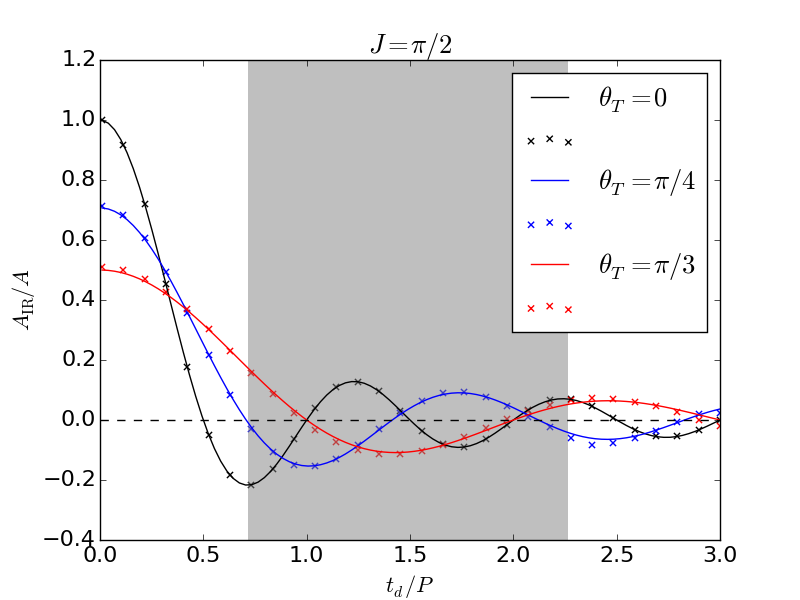
\includegraphics[scale=0.27]{figures/ch5/AIRplots/AIRoAUV_J1p5708_numin0_numx5_reclim2_TRHS} & 
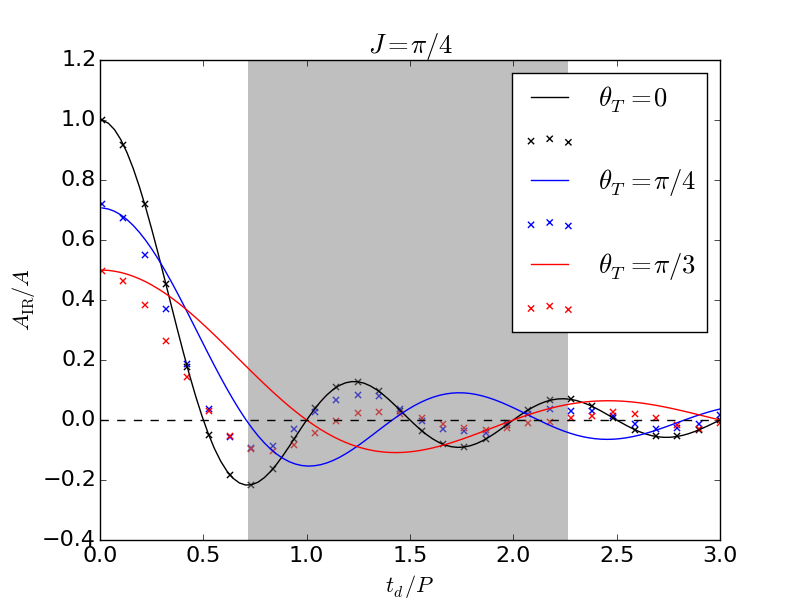
\includegraphics[scale=0.27]{figures/ch5/AIRplots/AIRoAUV_J0p785398_numin0_numx5_reclim2_TRHS} &
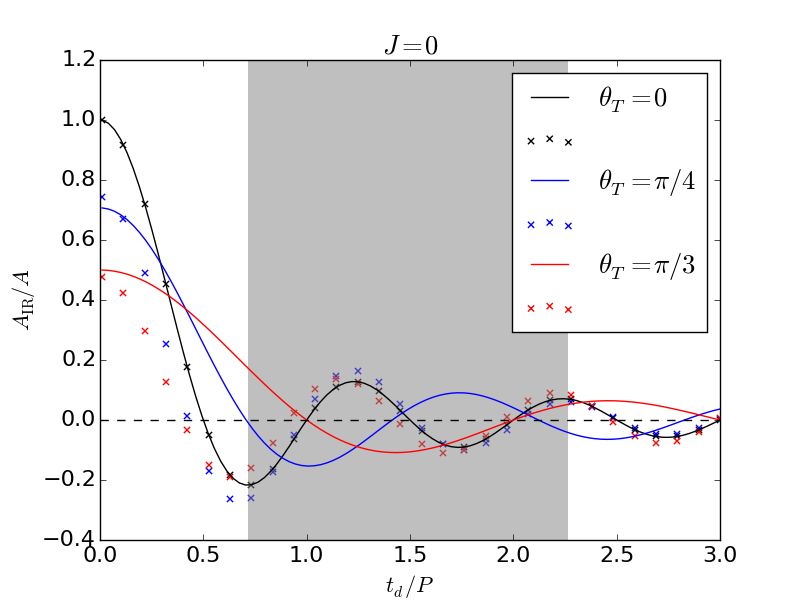
\includegraphics[scale=0.27]{figures/ch5/AIRplots/AIRoAUV_J0_numin0_numx5_reclim2_TRHS} 
\end{array}$
\end{center}
\caption{The amplitude of IR variability $A_{\rm{IR}}$ in terms of the UV/optical amplitude $A$ for a radially thin, dusty torus which absorbs all incident UV/optical radiation and emits it in IR. Each panel varies the opening angle $\theta_T$ of the torus for a different torus inclination angle $J$. The solid lines are the analytic solution Eq. (\ref{Eq:LIR_thT}) in the limit that $J=\pi/2$. The x's are the result of numerical calculations presented in \S \ref{S:Derivation}. The shaded region contains typical values of $t_d/P$ computed for the MBHB candidate PG 1302.}
\label{Fig:AIRoAUV_tr}
\end{figure}
%%%%%%%%%%%%%%%%%%%%%%%%%%%%%%%%%%%%%%%%%%%%%%%%


Figure \ref{Fig:AIRoAUVDop_tr} explores the dependence of IR variability
amplitude for the Doppler source with an edge-on binary inclination. The
behavior is similar to that of the isotropic case, with the $J=0$ and
$J=\pi/2$ panels bracketing the possible behavior. For near face-on binary
inclination, the IR variability amplitude can exceed the UV/optical amplitude,
this is discussed further below.

%%%%%%%%%%%%%%%%%%%%%%%%%%%%%%%%%%%%%%%%%%%%%%%%
%%% FIGURE: AIR/A Torus 1 DOP%%%
%%%%%%%%%%%%%%%%%%%%%%%%%%%%%%%%%%%%%%%%%%%%%%%%
\begin{figure}
\begin{center}$
\begin{array}{c c c}
%FISO and DOP 
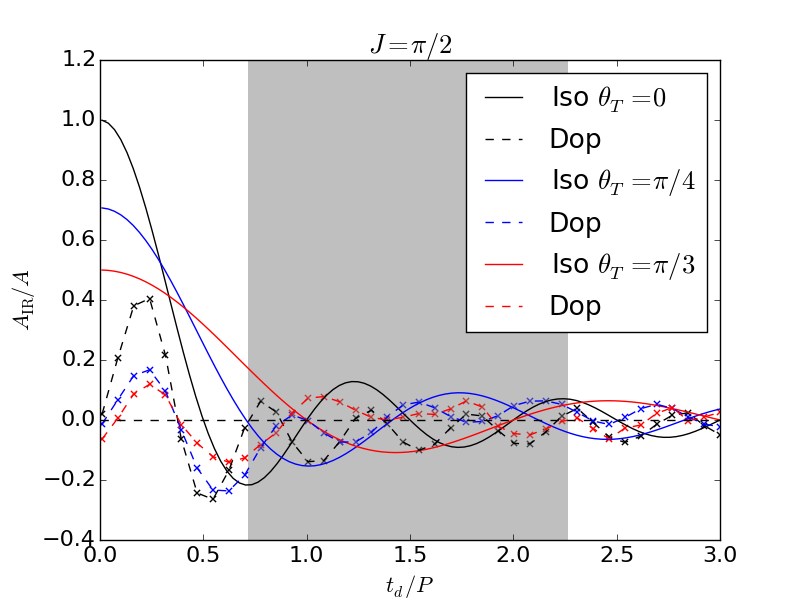
\includegraphics[scale=0.27]{figures/ch5/AIRplots/AIRoAUVDop_J1p5708_numin0_numx5_reclim2} &
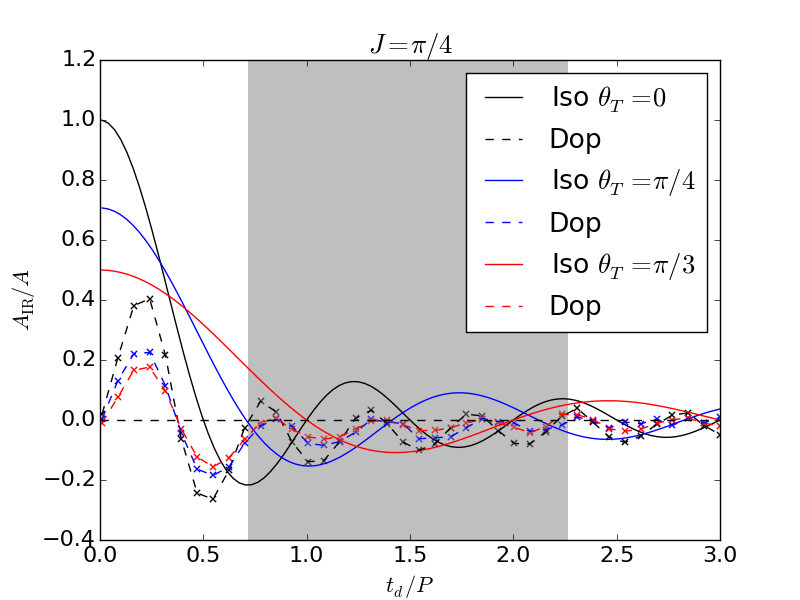
\includegraphics[scale=0.27]{figures/ch5/AIRplots/AIRoAUVDop_J0p785398_numin0_numx5_reclim2} &
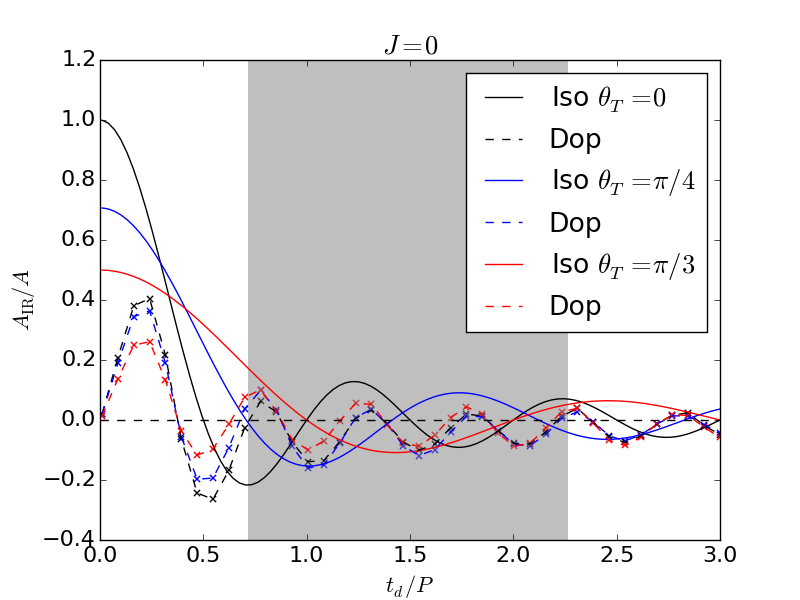
\includegraphics[scale=0.27]{figures/ch5/AIRplots/AIRoAUVDop_J0_numin0_numx5_reclim2} 
\end{array}$
\end{center}
%
\caption{The same as Figure \ref{Fig:AIRoAUV_tr}, but including the numerical
calculation of IR amplitudes for the Doppler boosted source with edge-on
binary inclination (x's). In each panel, the analytic, isotropic case for $J=
\pi/2$ is plotted for reference.}
%
\label{Fig:AIRoAUVDop_tr}
\end{figure}
%%%%%%%%%%%%%%%%%%%%%%%%%%%%%%%%%%%%%%%%%%%%%%%%






In Figure \ref{Fig:ShTor_DopvISO} we plot the IR (solid lines) and optical
light-curves (dashed lines) for various torus opening and inclination angles,
choosing a value of $t_d/P=0.6$. We recover the amplitudes of Figure
\ref{Fig:AIRoAUV_tr} and \ref{Fig:AIRoAUVDop_tr} and observe the expected
dimming of the IR light curves for larger torus opening angles. In both the
isotropic and Doppler cases, the phase lag of the IR to the UV/optical is
independent of the dust geometry parameters $J$ and $\theta_T$. In the
isotropic cases (left panels of Figure \ref{Fig:ShTor_DopvISO}) the one half
cycle phase shift between the $J=\pi/2$ and $J=0$ curves is consistent with
the corresponding signs of $A_{\rm{IR}}/A$ in Figure \ref{Fig:AIRoAUV_tr}; For
$J=\pi/2$, $A_{\rm{IR}}/A <0$ for the chosen $\theta_T$, while for $J=0$,
$A_{\rm{IR}}/A > 0$. See the previous section for a discussion of this phase
shift.





%%%%%%%%%%%%%%%%%%%%%%%%%%%%%%%%%%%%%%%%%%%%%%%%
%%% FIGURE: Sphere IR light curves ISO vs Dop%%%
%%%%%%%%%%%%%%%%%%%%%%%%%%%%%%%%%%%%%%%%%%%%%%%%
\begin{figure}
\begin{center}$
\begin{array}{c c}
%FISO and DOP  vary Rin
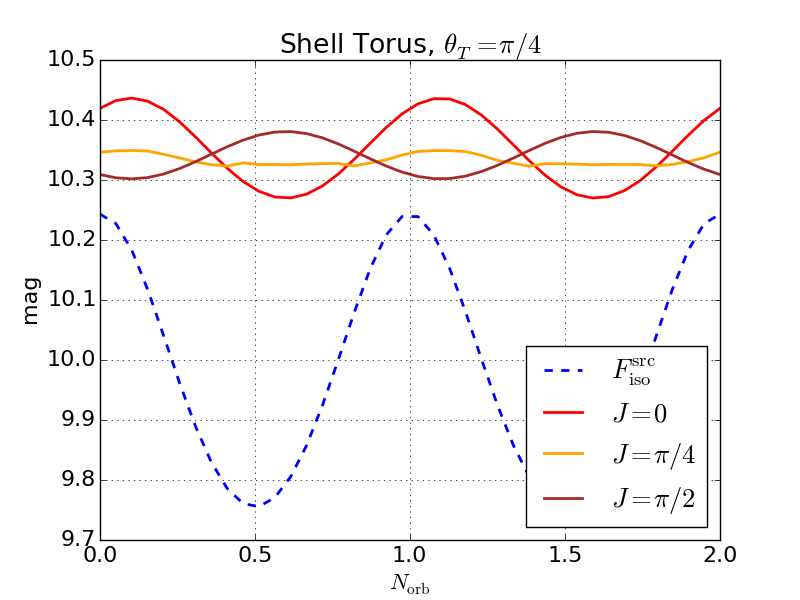
\includegraphics[scale=0.33]{figures/ch5/ShTor_Thin/FISO_ShTor_Thin_nrm0__Rin2p73218e+18_Inc0_thetaT0p785398_VaryJ_numin0_numx6} & 
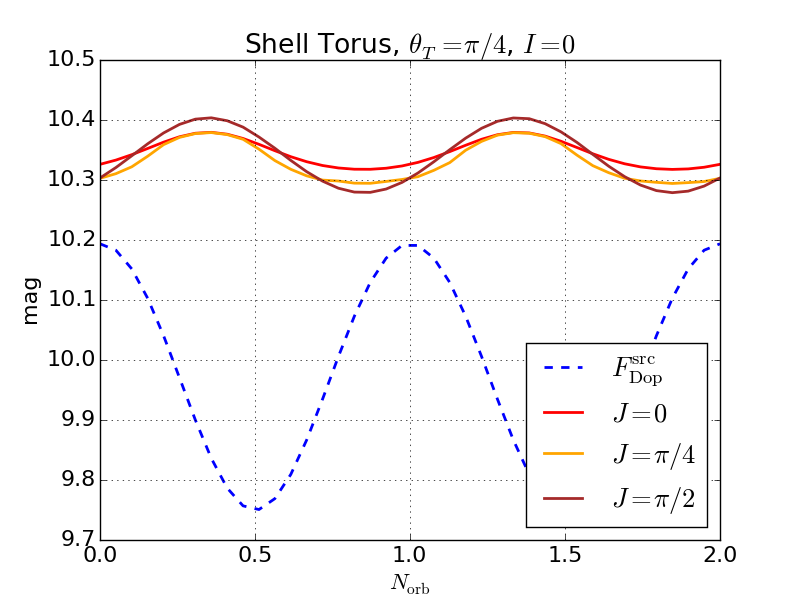
\includegraphics[scale=0.33]{figures/ch5/ShTor_Thin/FDop_ShTor_Thin_nrm0__Rin2p73218e+18_Inc0_thetaT0p785398_VaryJ_numin0_numx6} \\
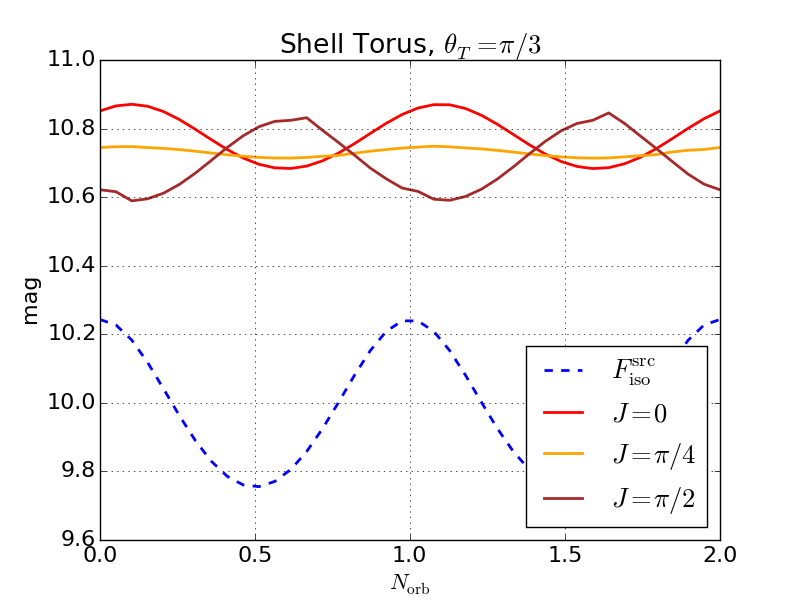
\includegraphics[scale=0.33]{figures/ch5/ShTor_Thin/FISO_ShTor_Thin_nrm0__Rin2p73218e+18_Inc0_thetaT1p0472_VaryJ_numin0_numx6} &
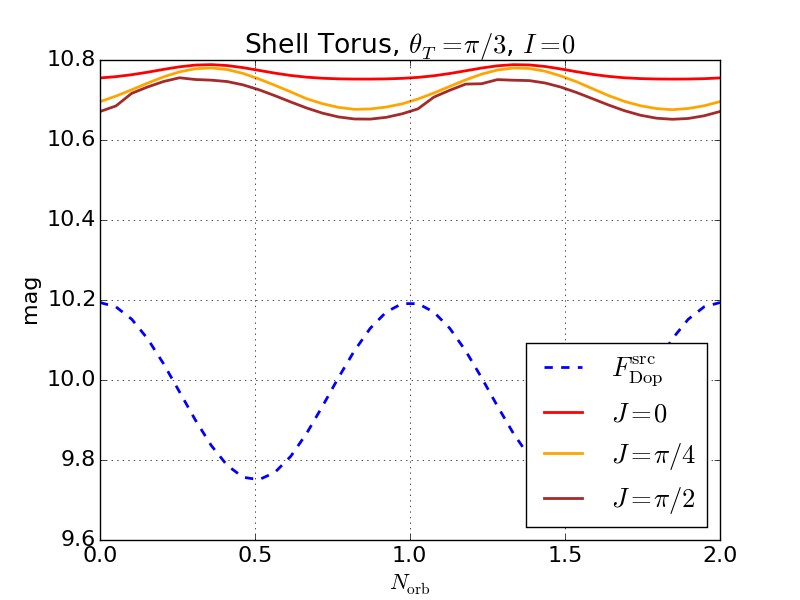
\includegraphics[scale=0.33]{figures/ch5/ShTor_Thin/FDop_ShTor_Thin_nrm0__Rin2p73218e+18_Inc0_thetaT1p0472_VaryJ_numin0_numx6}
\end{array}$
\end{center}
%
\caption{The same as Figure ref{Fig:SphDopvISO} but for the torus dust shell
model. Here $R_d = 0.6 R_0$, each panel plots IR light curves for different
torus inclination angles, and for a chosen torus opening angle $theta_T$. The
left panel assumes an isotropic central source while the right panels assume a
Doppler boosted source.}
%
\label{Fig:ShTor_DopvISO}
\end{figure}
%%%%%%%%%%%%%%%%%%%%%%%%%%%%%%%%%%%%%%%%%%%%%%%%



Finally, we explore the effects of binary inclination in the torus dust model.
With the freedom to orient the binary plane relative to a non-spherical dust
structure through parameters $I$ and $J$ (for $\theta_T \neq 0$), the
possibility of generating IR variability with no observed UV variability
arises. Figure \ref{Fig:ShTor_VarI} demonstrates that when the binary is
face on, there is no observed UV/optical variability (\textit{e.g.} Eq
\ref{Eq:vlos}), but IR variability still persists. For the spherical model,
a face-on binary generated zero IR variability because no time
changing emission was generated between the front and back hemispheres of the dust sphere.
This back front symmetry is broken in the case of a torus dust shell, as
long as $J\neq 0$ and $J\neq \pi/2$.




%%%%%%%%%%%%%%%%%%%%%%%%%%%%%%%%%%%%%%%%%%%%%%%%
%%% FIGURE: Sphere IR light curves ISO vs Dop%%%
%%%%%%%%%%%%%%%%%%%%%%%%%%%%%%%%%%%%%%%%%%%%%%%%
\begin{figure}
\begin{center}
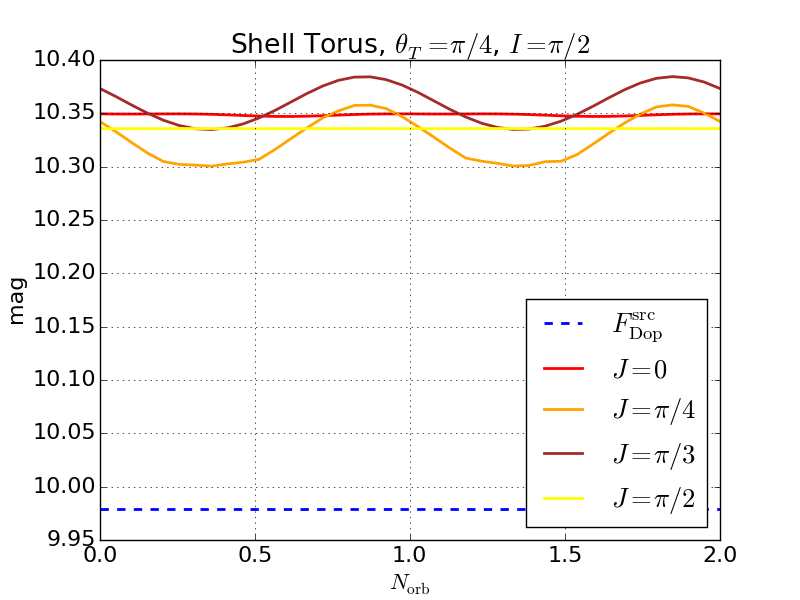
\includegraphics[scale=0.33]{figures/ch5/ShTor_Thin/FDop_ShTor_Thin_nrm0__Rin2p73218e+18_Inc1p5708_thetaT0p785398_VaryJ_numin0_numx6} 
\end{center}
%
\caption{The same as Figure \ref{Fig:ShTor_DopvISO} but for a face-on binary
inclination. For all but extreme torus inclinations $J=0, \pi/2$,
significant IR variability persists even when no UV/optical variability is
observed.}
%
\label{Fig:ShTor_VarI}
\end{figure}
%%%%%%%%%%%%%%%%%%%%%%%%%%%%%%%%%%%%%%%%%%%%%%%%














\begin{table*}
\caption{Parameters of the model and their fiducial values if not otherwise stated in the text.}
\label{Table:params}
%
\rotatebox{90}{
%
%\begin{center}
\begin{tabular}{ c | c | c | c}
        Parameter         & Meaning     & Fiducial Value   &   Notes \\
                   \hline 
                  Binary Parameters &  & \\
                  \hline    
$L^0$                & Bolometric source luminosity            & $6.78\times10^{46}$  erg s$^{-1}$    & PG 1302 value\\
$\bar{\alpha}$       &Source averaged spectral index            &  0.0  & \\
%$M$                                     & Total Mass        & $10^{9.1} \rightarrow 10^{9.4} \Msun $      \\
$\Omega$             & Orbital frequency                        & $2 \pi c/R_0 $     & \\
%$q$                                       & Mass ratio           & $\lsim 0.1$    \\
$\beta$              & Boost velocity$/c$                       & $0.068$   & Inferred from binary mass,\\
&&& period, and mass ratio. \\
$I$                                      & Inclination                          &  $0$  & $0$ is edge-on \\%Inferred from $\beta$ and variability magnitude   \\
                   \hline   
                  Dust Parameters &  & \\
                  \hline    
$\Rin$               &  Inner edge of dust                                      & $\chi R_0 = \chi 0.9 \sqrt{\epsilon/0.1}$ pc      & $R_0=$Sublimation radius for \\
&&& Graphites around PG 1302\\
%{$n_0$}            &  Density normalization                                 & $(p-1) (\pi a^2_{\eff} \Rin)^{-1}$    &       \\
%{$p$}                &  Density exponent                                    & 2.0                       &   $n_d(r) = n_0 \left( \Rin/r \right)^{p}$    \\
{$J$}                &  Torus inclination                                       & $\pi/2$                       &   0 obstructed; $\pi/2$ un-obstructed \\
{$\theta_T$}     &  Torus opening angle                                   & $\pi/4$                     &   0 is a dust sphere\\
%$\Rout$            &  Outer edge of dust                                   & $10\Rout$                     & weak dependence for $p>0$     \\
$k$             &  Absorption/emission efficiency exponent                      & 1                             &   \\
$\nu_0$     & Efficiency cutoff frequency                           &    $c/(2 \pi a_{\rm{eff}})$           & $Q_{\nu} = \rm{min}\left[ \left( \nu/ \nu_0 \right)^{k}, 1\right]$    \\
$a_{\rm{eff}}$  &  Grain size                                               &  $0.16$ $\mu$m                    &  Set by $\nu_0$       
 \label{Table:params}
 \end{tabular}
 %
 }
 %
%\end{center}
\end{table*}













\section{Discussion and Conclusion}
\label{S:Discussion}
We summarize our key results and discuss their implications for MBHBs.

\begin{enumerate}
\item{
\textbf{The amplitude of IR variability} relative to UV/optical modulation i s
a function of the ratio of dust light crossing time to variability period
$t_d/P$. The IR amplitude depends on the inclination and opening angles of the
dust torus for an isotropic source in addition to the binary inclination to
the line of sight for a Doppler boosted source. Generally the IR amplitude
falls to zero for $t_d/P \gg 1$, and approaches that of the UV/optical
continuum for $t_d/P \rightarrow 0$ in the isotropic case, while the Doppler
case obtains peak amplitude at $t_d/P \sim 0.25$ and falls to zero for $t_d/P
\rightarrow 0$.


Using Eq. (\ref{Eq:Rd}), we can relate the value of $t_d/P$ to the mass of the
binary (through the Eddington limit) and the variability period,
\begin{equation}
t_d/P \sim 0.7 \left(\frac{P}{4 \rm{yr} } \right)^{-1} \left(\frac{M}{10^9 \Msun } \right)^{1/2}.
\end{equation}
Contours of $t_d/P$ are overlaid in Figure \ref{Fig:boostParams}. From Figure
\ref{Fig:boostParams} and Figure \ref{Fig:AIRoAUV_sp}, we conclude that, for
isotropic sources, long period, low mass binaries would generate the largest
IR modulations. If the variations are due to the Doppler boost however, low
mass binaries on long period orbits create weak UV/optical variations to start
with, and more intermediate masses and binary periods are favored for
detection of variability in the IR. The range of values of $t_d/P$ relevant
for the MBHB candidate PG 1302 (for $\epsilon =0.1 \rightarrow 1$ in Eq.
(\ref{Eq:Rd})) are shaded grey in Figures \ref{Fig:AIRoAUV_sp}, \ref{Fig:Qvon},
\ref{Fig:AIRoAUV_tr}, and \ref{Fig:AIRoAUVDop_tr}. }

%
\item{ 
\textbf{The phase lag of IR variability} to UV/optical variability depends
only on the ratio $t_d/P$ for both Doppler and isotropic sources. However,
each source produces a different phase lag which could aid in differentiating
the two types of variability and should be considered when simply relating an
IR time lag with the light travel time across the dust reverberation region.

We also point out that, while IR variability from isotropic sources is lagged by
a fraction $t_d/P$ of one variability cycle, there will be an additional half
cycle phase shift for light curves which are symmetric about their average
(sinusoids). Whether this phase shift occurs depends on the value of $t_d/P$
(see Eq. \ref{Eq:LIR_thT}) and is important for determining the size of the
emitting dust region through IR phase lags. } 
%
\item{
\textbf{Orphan IR variability} can occur for Doppler sources which are nearly
face-on (so we do not see the UV/optical variability), but are surrounded by a
dust torus which is not symmetric between the front and back of the Doppler
boost source. Such orphan IR periodicity in quasars could be a smoking gun
signature of Doppler boosted MBHBs at high inclination to the line of sight,
and would not as yet been identified in optical searches such as those carried
out by \cite{Graham+2015b} and \citep{Charisi+2016}. }

\end{enumerate}


 

We list caveats and possible extensions to this work: 
\begin{itemize}

\item We have considered geometrically thin dust models which are optically
thin to their own emission. Dust models which consider the finite radial
extent of the dust and the possibility of IR absorption by dust are being
considered in forthcoming work. Furthermore, dusty tori are thought to be
clumpy \citep[\textit{e.g}][and references therein]{Netzer:2015:rev}. Future,
more sophisticated dust models and radiative transfer may reveal interesting
new diagnostics.



\item We have assumed a uniform distribution of dust grain sizes.  In reality
there may be a distribution of dust grain species and sizes.


\item 
We have assumed that the relative location of the emitting secondary is small
compared to the dust torus inner radius. Because of finite light travel times,
the relative motion of the binary with respect to the dusty torus will become
important on the level of the ratio of the binary separation and the size of
the IR reprocessing region (the dust). The ratio of binary separation to
torus inner edge is
\begin{equation}
\frac{a}{R_d} \simeq 0.016\ \epsilon_{0.1} \left(\frac{M}{10^9 \Msun}\right)^{-1/6}  \left(\frac{P}{5 \rm{yr}}\right)^{2/3}  \left(\frac{T}{1800 \rm{K}}\right)^{2.6},
\label{Eq:aORd}
\end{equation}
telling us that the impact of binary orbital motion on the time lags of
reprocessed light will be most important for the lowest mass binaries with the
longest periods, and contribute on at most the $1.6 \%$ level for the
fiducial values taken here for a PG1302-like binary. Because the dependence on
mass is weak, and 5 years is a current upper limit on observed binary periods
discovered in EM time-domain surveys \citep[\textit{e.g.}][]{Graham+2015b}, it
is safe to assume that the effect of binary orbital motion is a $\lsim 2\%$
effect.

It will be important to take this effect into account for modeling the effects
of Doppler boosted emission on broad line regions around MBHBs, the subject of
future work.


\item We assume a binary on a circular orbit in the case of a Doppler source.
Some hydrodynamical models of the binary interaction with a gas disk predict
that large binary eccentricities can be excited \citep{Roedig:2011:eccevo}.
Such binary eccentricities will change the shape of the optical and hence the
IR light curves predicted here.





 \item If grains can re-form on a timescale shorter than a binary orbital time, the inner sublimation radius will change periodically with the changing central source flux. From Eq. \ref{Eq:Rd}, the change in dust sublimation due to the changing observed flux variations $\delta F$ is
 \begin{equation}
 \frac{\delta R_d}{R_d} = \frac{1}{2} \frac{\delta F}{F}
 \end{equation}
which could result in changes to the inner dust radius of a few to $\sim 10 \%$ for typical Doppler flux variations.


\item General relativistic time lags and precession could become important. 
%http://arxiv.org/abs/1604.02148


\end{itemize}


\section{Conclusions}
\label{S:conclusions}
We have developed a model to compute IR light curves from isotropically
emitting and anisotropically emitting Doppler boosted MBHBs. The latter,
describing reverberation from a lighthouse-like central source is presented
here for the first time. We show that the phase, amplitude, and average
brightness of reverberated IR radiation is dependent on the ratio of light
travel time across the emitting dust region as well as dust geometric
properties, and in the case of Doppler boosted emission, the relative
inclination of binary orbital plane and dust torus. 

Future work will expand these models to incorporate more sophisticated dust
structures and radiative transfer. These along with the models and intuition
developed here will be applied to fit the IR light curves of the growing list
of MBHB candidates \citep{Graham+2015b, Charisi+2016, Jun:2015}. This will aid
in the interpretation of such sources as MBHBs, and also illuminate their
surrounding, dusty environments.



This model will not only be useful for interpreting the nature of existing
MBHB candidates, but could help to discover more. If the binary's orbit is
highly inclined to the line of sight, but not to the dust structure, then an
imprint of Doppler boosting will not appear in the optical and UV, but it will
appear in the IR. This motivates a search for such Orphan-IR Doppler imprints.



\renewcommand\thesection{\thechapter.\arabic{section}}